\renewcommand{\thechapter}{\arabic{chapter}}
\setcounter{chapter}{5}

\chapter{Amélioration du diagnostic image}
\label{chap:chapter_6}
\chapterintro
Les expérimentations conduites lors du précédent chapitre ont tenté d'apporter une première réponse pour la séparation des images de \acrlong{mcr} et menées selon les annotations saines, bénignes ou encore malignes. Pour cela, ce travail s'est intéressé aux méthodes permettant de caractériser au mieux les aspects de texture de ces images par l'extraction de caractéristiques pertinentes mais également aux méthodes de classification permettant la meilleure séparation des images selon les précédentes annotations.\par

Néanmoins, ces méthodes abordent la problématique par une compréhension globale des images de \acrlong{mcr}, dont le principe même est considéré comme une limitation dans ce nouveau chapitre. Ainsi, de nouveaux schémas sont considérés afin d'améliorer le diagnostic de ces images. Des méthodes exploitant le principe de résolution multiple, de fenêtre glissante, ou encore exploitant les \acrlong{cnn} par réglage fin de bout en bout sont mises en œuvre dans ce nouveau chapitre.\par

\newpage

\section{Méthodologie}
Lors du précédent chapitre, diverses approches ont été proposées afin de comprendre les composants essentiels d'une image dans son intégralité, et de permettre ainsi la séparation des éléments \textbf{sains}, \textbf{bénins} et \textbf{malins}. Cette approche suppose que l'information extraite afin de caractériser ces images est suffisante pour permettre une séparation selon les trois précédentes annotations. Cette hypothèse n'est que partiellement juste puisqu'une même image de la modalité de \gls{mcr} peut comporter divers types de tissus selon ces trois annotations, dont la hiérarchie d'inclusion entre annotations est visible sur la \Cref{fig:scheme_image_improvement_annotations_hierarchy}.\par

\begin{figure}[H]
    \centering
    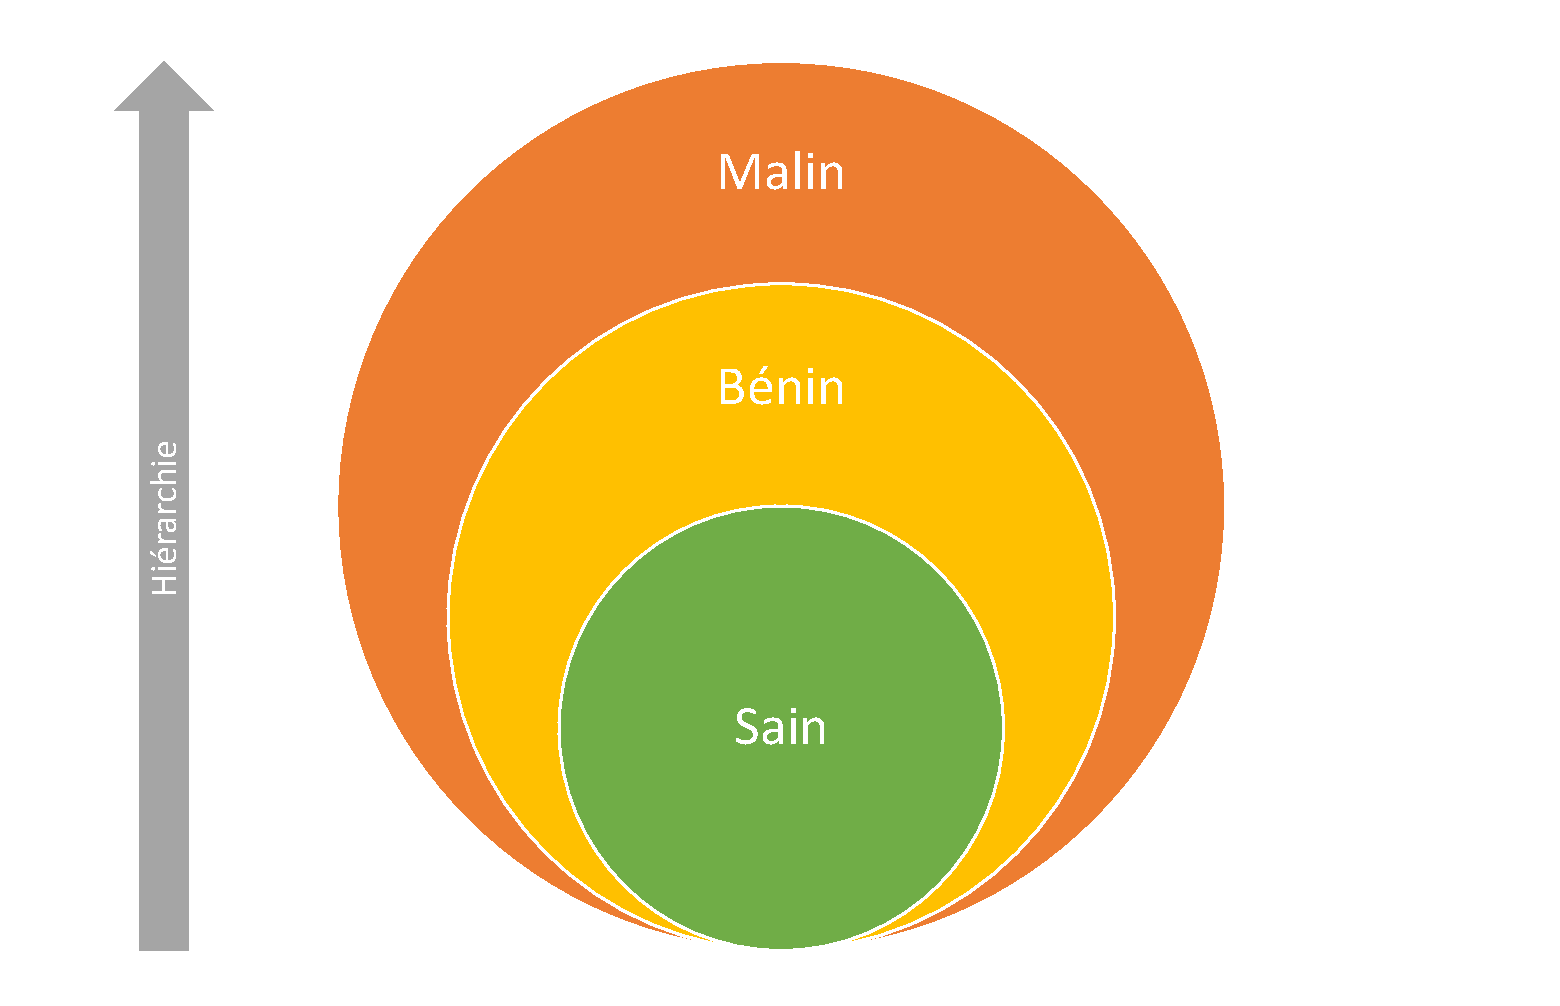
\includegraphics[width=0.6\textwidth]{contents/chapter_6/resources/scheme_image_improvement_annotations_hierarchy.pdf}
    \caption{Schéma représentatif de la relation hiérarchique entre les annotations. Les images malignes peuvent ainsi contenir des tissus bénins et sains~;~Les images bénignes peuvent contenir des tissus sains~;~Les images saines ne contiennent que des tissus sains.}
    \label{fig:scheme_image_improvement_annotations_hierarchy}
\end{figure}\par

Dans ce nouveau chapitre dédié à l'amélioration du diagnostic de l'image, les observations du \Cref{chap:chapter_5} sont reprises, en privilégiant notamment l'utilisation de la \textbf{normalisation par Minimum / Maximum} et le \textbf{modèle \gls{svm} à noyau linéaire}. Les représentants les plus performants des méthodes d'extraction de caractéristiques sont également conservés dans ce travail, dont~:
\begin{itemize}
    \item pour la \textbf{catégorie de méthodes spatiales}, les caractéristiques définies par Haralick~\al{Haralick1973},
    \item pour la \textbf{catégorie de méthodes fréquentielles}, les caractéristiques sur base d'extraction en ondelettes,
    \item pour la \textbf{catégorie de méthodes de transfert de connaissances}, l'architecture ResNet-50 associée à une couche de Global Pooling - Moyenne.
\end{itemize}\par

Ainsi, des schémas alternatifs sont envisagés afin d'extraire une information nécessaire à la séparation des données de la modalité de \gls{mcr}. Ce chapitre débute par la présentation de \textbf{méthodes multi-échelle}, en supposant que l'information comporte plusieurs niveaux d'interprétations. Puis, s'ensuit la description de \textbf{méthodes par fenêtre glissante} pour extraire localement une information propre aux tissus. Afin d'étendre ce principe d'approche locale, ce travail s'intéresse à l'utilisation du \textbf{réglage fin sur des \gls{cnn}}. Enfin, ce chapitre propose \textbf{une analyse des résultats} issus de ces diverses méthodes, lesquels aboutissent à \textbf{une discussion} permettant d'approfondir ces résultats.\par
\clearpage

\section{Approche multi-échelle}
Comme évoqué précédemment, les traitements réalisés jusqu'alors ne permettent qu'une compréhension globale de l'image. Cette vision de l'extraction de caractéristiques peut être erronée si l'on suppose une interprétation de l'image à divers niveaux de compréhension.\par

C'est ainsi que des hypothèses de compréhension de l'image à échelles multiples ont émergé, bien que peu relatées dans la littérature. Ces approches ont été employées à différentes fins~:
\begin{inlinerate}
    \item de détection de frontières dans un contexte d'images naturelles~\cite{Ren2008},
    \item de segmentation d'images~\cite{DosSantos2012,Arbelaez2014},
    \item de détection d'objets~\cite{Felzenszwalb2008} ou d'actions~\cite{Pedersoli2011},
    \item ou encore de classification d'images médicales~\cite{Alsaih2016,Tang2017}.
\end{inlinerate} En termes de traitements appliqué à la modalité de \gls{mcr}, le travail de Wiltgen~\al{Wiltgen2008} semble être le plus proche de la thématique de ce chapitre et propose entre autres des méthodes de prise en charge par échelles multiples. Ainsi, cette section est scindée en deux parties respectives, avec d'une part l'application de ce principe à la décomposition en ondelettes et d'autre part l'application de ce principe à des techniques d'extractions spatiales.\par 

\subsection{Décomposition en ondelettes multi-échelle}
La première approche présentée se base sur la décomposition en ondelettes multi-échelle. En effet, ce principe a été démontré comme judicieux dans de nombreux domaines impliquant l'analyse d'images~\cite{Carvalho2004}. Cette décomposition peut être effectuée sous la forme de schémas qualifiés soit de \textbf{diadique}, soit de \textbf{pyramidal}. Ces deux modes sont schématisés sur la \Cref{fig:scheme_image_improvement_dwt_decomposition}. L'un des articles de référence de ce travail préconise l'utilisation du schéma de décomposition diadique pour l'extraction de caractéristiques de texture sur images de \gls{mcr}~\cite{Wiltgen2008}. Pour cela, les auteurs se focalisent sur l'utilisation d'une \textbf{ondelette mère de Daubechies} et emploient cette transformée à cinq niveaux de détails successifs sous forme d'arbre diadique. Les mesures associées à chaque bande de fréquences de la transformée sont les mêmes que dans le \Cref{chap:chapter_5} et se basent sur l'extraction de l'\textbf{écart-type}, de l'\textbf{énergie} et de l'\textbf{entropie} pour un total de \textbf{39 caractéristiques}. Suite aux résultats obtenus et présentés dans le \Cref{chap:chapter_5}, ce procédé est également évalué selon \textbf{l'ondelette mère de Haar}.\par

\begin{figure}[H]
    \centering
    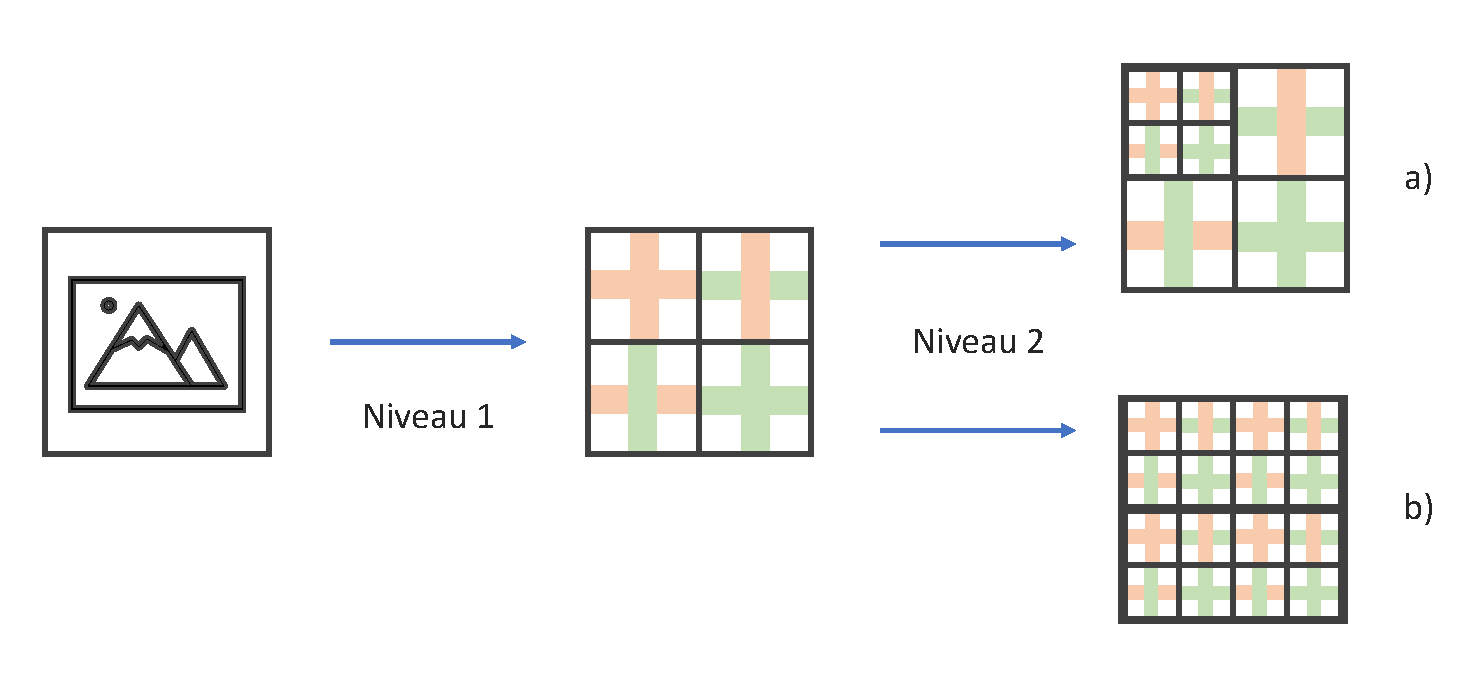
\includegraphics[width=\textwidth]{contents/chapter_6/resources/scheme_image_improvement_dwt_decomposition.pdf}
    \caption{Schématisation des deux principaux types de décomposition successive par ondelettes. En a), schéma de décomposition multi-échelle en ondelettes dit \textbf{diadique}~;~En b), schéma de décomposition multi-échelle en ondelettes dit \textbf{pyramidal}.}
    \label{fig:scheme_image_improvement_dwt_decomposition}
\end{figure}\par

La seconde méthode sur laquelle ce travail prend appui est une extension de la transformée en ondelettes de l'article de Wiltgen~\al{Halimi2017a}. Ainsi, cette nouvelle méthode reprend la précédente décomposition selon un schéma diadique, et en modifie le \textbf{nombre de décompositions à quatre niveaux}, au lieu des cinq initialement prévus. Selon cette même méthode, une loi normale généralisée centrée, dont la densité de probabilité $f$ est décrite par l'\Cref{eq:image_improvement_ggd}, est ajustée à la distribution de valeurs de chaque niveau de décomposition. Enfin, les auteurs de l'étude ne retiennent comme caractéristiques que \textbf{les paramètres d'échelle $\alpha$ et de forme $\beta$} de cette loi normale généralisée pour un total de \textbf{24 caractéristiques}, et où $\Gamma$ représente la fonction gamma.\par

\begin{equation}
    f(x)= \frac{\beta}{2\alpha\Gamma(1/\beta)} e^{-\left(|\frac{x}{\alpha}|\right)^\beta}
    \label{eq:image_improvement_ggd}
\end{equation}

Afin de gérer ces diverses caractéristiques, ce travail s'emploie à l'utilisation d'un \textbf{modèle de type \gls{svm} à noyau linéaire}, démontré empiriquement efficace pour la classification de données fréquentielles lors du \Cref{chap:chapter_5}. Les hyperparamètres employés afin de tirer le meilleur parti de ce modèle sont listés dans la \Cref{tab:parameters_image_improvement_multiscale_frequency}. L'implémentation du modèle \gls{svm} utilisé provient de la bibliothèque logicielle \textit{Scikit-learn}~\cite{pedregosa2011}.\par

\begin{table}[H]
    \centering
    \begin{tabular}{lll}
        \toprule
        \textbf{Modèle}                                 & \textbf{Hyperparamètres}  & \textbf{Valeurs}                          \\ \midrule
        \gls{svm} - Noyau linéaire                      & C                         & [0,001, 0,01, 0,1, 1, 10, 100, 1000]      \\ 
        \bottomrule 
    \end{tabular} 
    \caption{Table reprenant le modèle de classification et ses hyperparamètres employés sur les caractéristiques issues de la décomposition en ondelettes multi-échelle.}
    \label{tab:parameters_image_improvement_multiscale_frequency}
\end{table}\par

Les étapes de transformée en ondelettes et la décomposition en ondelettes multi-échelle de cette expérimentation sont réalisées à l'aide de la bibliothèque logicielle \textit{PyWavelets}~\cite{lee2006}. Quant aux opérations d'ajustement de la loi généralisée, celles-ci s'appuient sur la bibliothèque logicielle \textit{SciPy}~\cite{Virtanen2020}. Ces expérimentations basées sur la décomposition en ondelettes multi-échelle sont recensées dans la \Cref{tab:wavelet_image_improvement_multiscale_nb_features} ainsi que leurs nombres de caractéristiques associées à chacune d'entre elles.\par

\begin{table}[h]
    \centering
    \begin{tabular}{ll}
        \toprule
        \textbf{Méthode}                                    & \textbf{Nombre de caractéristiques}   \\ \hline
        Ondelettes - Haar                                   & 39 (13 $\times$ 3)                    \\ \hline
        Ondelettes - Daubechies / Wiltgen~\cite{Wiltgen2008}& 39 (13 $\times$ 3)                    \\ \hline
        Halimi~\cite{Halimi2017a}                           & 24 (12 $\times$ 2)                    \\
        \bottomrule
    \end{tabular}
    \caption{Liste des méthodes de décomposition en ondelettes multi-échelle et leur nombre de caractéristiques extraites associées.}
    \label{tab:wavelet_image_improvement_multiscale_nb_features}
\end{table}\par
\clearpage

\subsection{Décomposition spatiale multi-échelle}
Lors de la précédente sous-section, les approches par décomposition en ondelettes multi-échelle ont été présentées. Toujours dans cette optique d'approche multi-échelle, divers travaux se sont orientés afin de permettre une classification d'images médicales sur la base d'extraction de caractéristiques spatiales~\cite{Alsaih2016,Tzalavra2016}. Les prochaines étapes s'inspirent de ces travaux mais également des conclusions apportées par le \Cref{chap:chapter_5} sur l'extraction de caractéristiques spatiales et par transfert de connaissances. Ainsi, sont mis en œuvre deux processus multi-échelle dans ce chapitre, présentés lors des prochains paragraphes.\par

La première méthode proposée se base sur une approche de type fusion de caractéristiques avant l'étape de classification, déjà rencontrée dans des travaux à but similaire~\cite{Pedersoli2011,Alsaih2016}. Afin de permettre l'agrégation de ces caractéristiques, une \textbf{normalisation par Minimum / Maximum} associée à un \textbf{modèle \gls{svm} à noyau linéaire} est employée, démontré efficace de manière empirique lors du \Cref{chap:chapter_5} et robuste dans des contextes à fortes dimensions. À nouveau, l'implémentation du modèle \gls{svm} employé dans ce travail provient de la bibliothèque logicielle \textit{Scikit-learn}~\cite{pedregosa2011} et les hyperparamètres utilisés par ce modèle sont recensés dans la \Cref{tab:parameters_image_improvement_models_multiscale_spatial}. Le principe de fonctionnement de cette première méthode est schématisé sur la \Cref{fig:scheme_image_improvement_multiscale_features}.\par

\begin{figure}[H]
    \centering
    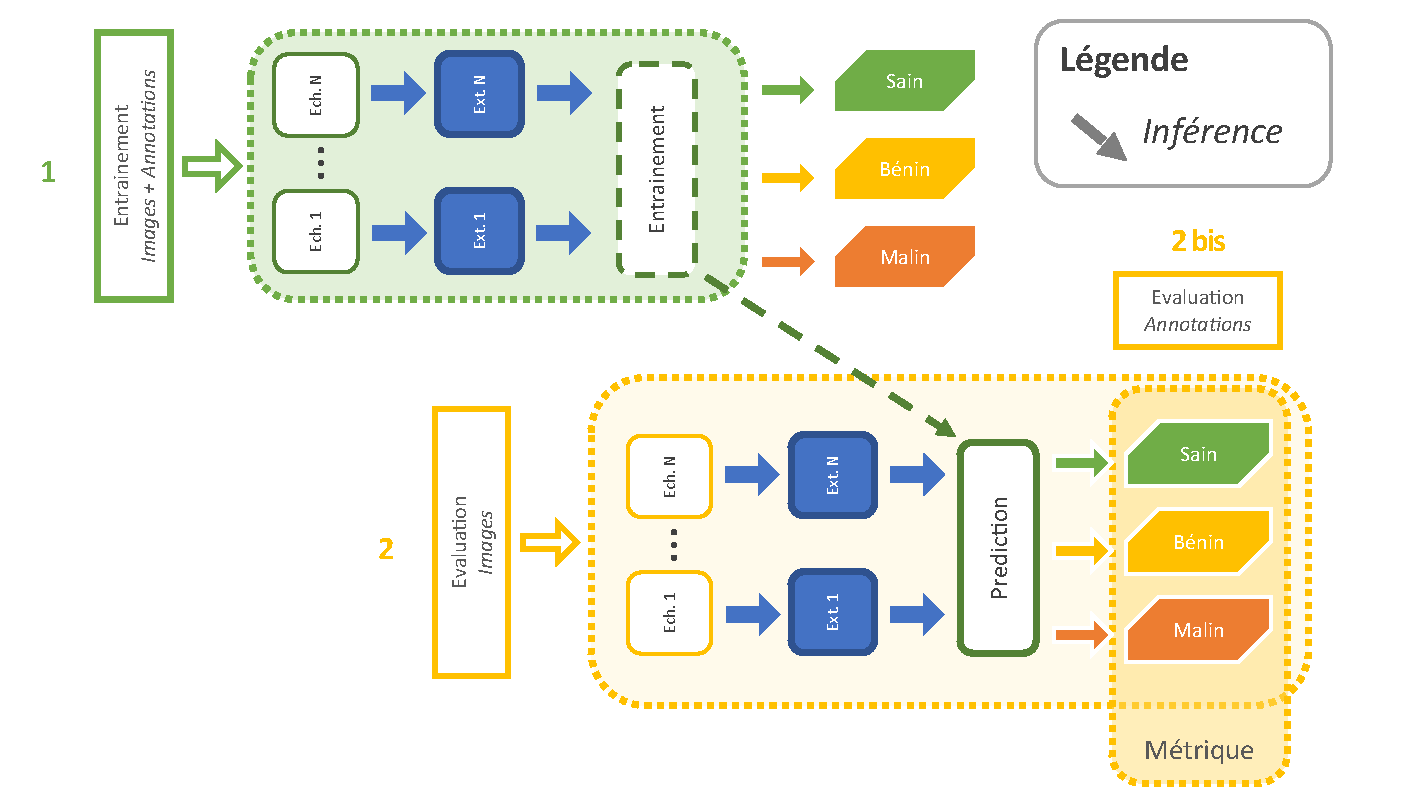
\includegraphics[width=0.9\linewidth]{contents/chapter_6/resources/scheme_image_improvement_multiscale_features.pdf}
    \caption{Schéma de représentation du système multi-échelle, sur la base d'une extraction à diverses échelles puis par l'agrégation des caractéristiques avant la procédure de classification.}
    \label{fig:scheme_image_improvement_multiscale_features}
\end{figure}\par

La seconde méthode correspond à un schéma en deux temps, dans lequel chaque modèle de prédiction est spécialisé à une échelle spatiale précise. À cette fin, est employée pour chacune de ces échelles une \textbf{normalisation par Minimum / Maximum} associée à un \textbf{modèle de type \gls{svm} à noyau linéaire} pour les raisons évoquées précédemment, dont les hyperparamètres sont recensés dans la \Cref{tab:parameters_image_improvement_models_multiscale_spatial}. Ce faisant, il est alors nécessaire de réunir ou \textbf{fusionner} ces informations en une unique décision à l'aide d'\textbf{un vote à la majorité}~\cite{TinKamHo1994,Lam1997}, dont le principe ne nécessite aucune phase d'entraînement. Cette technique est ainsi employée~:
\begin{inlinerate}
    \item sur les \textbf{scores} définis par l'ensemble $\mathbf{R}$,
    \item mais également sur les \textbf{décisions} définies par l'ensemble $\mathbf{N}$.
\end{inlinerate} Une première méthode est mise en place à l'aide d'\textbf{une fonction de moyenne appliquée aux scores}, de laquelle est extrait le score le plus élevé. Ce schéma permet de notifier d'\textbf{une tendance globale} d'une classe par rapport aux autres. Une seconde méthode est mise en place à l'aide d'\textbf{une fonction de maximum appliquée aux scores}, de laquelle est extrait le score le plus élevé. Ce schéma permet d'isoler la classe recueillant la confiance de prédiction la plus élevée. Enfin, la dernière méthode est mise en place par recensement de la classe qui a recueilli \textbf{le plus grand nombre de décisions}. Le processus global de cette expérience est présenté sur la \Cref{fig:scheme_image_improvement_multiscale_decision}.\par

\begin{table}[H]
    \centering
    \begin{tabular}{lll}
        \toprule
        \textbf{Modèle}                                 & \textbf{Hyperparamètres}  & \textbf{Valeurs}                          \\ \midrule
        \gls{svm} - Noyau linéaire                      & C                         & [0,001, 0,01, 0,1, 1, 10, 100, 1000]      \\ 
        \bottomrule 
    \end{tabular} 
    \caption{Table recensant les paramètres du modèle de classification employé pour réaliser la prédiction sur des caractéristiques spatiales multi-échelle. Ce modèle associé à ces hyperparamètres est employé pour la classification par échelle mais également pour l'agrégation des multiples échelles.}
    \label{tab:parameters_image_improvement_models_multiscale_spatial}
\end{table}\par

\begin{figure}[H]
    \centering
    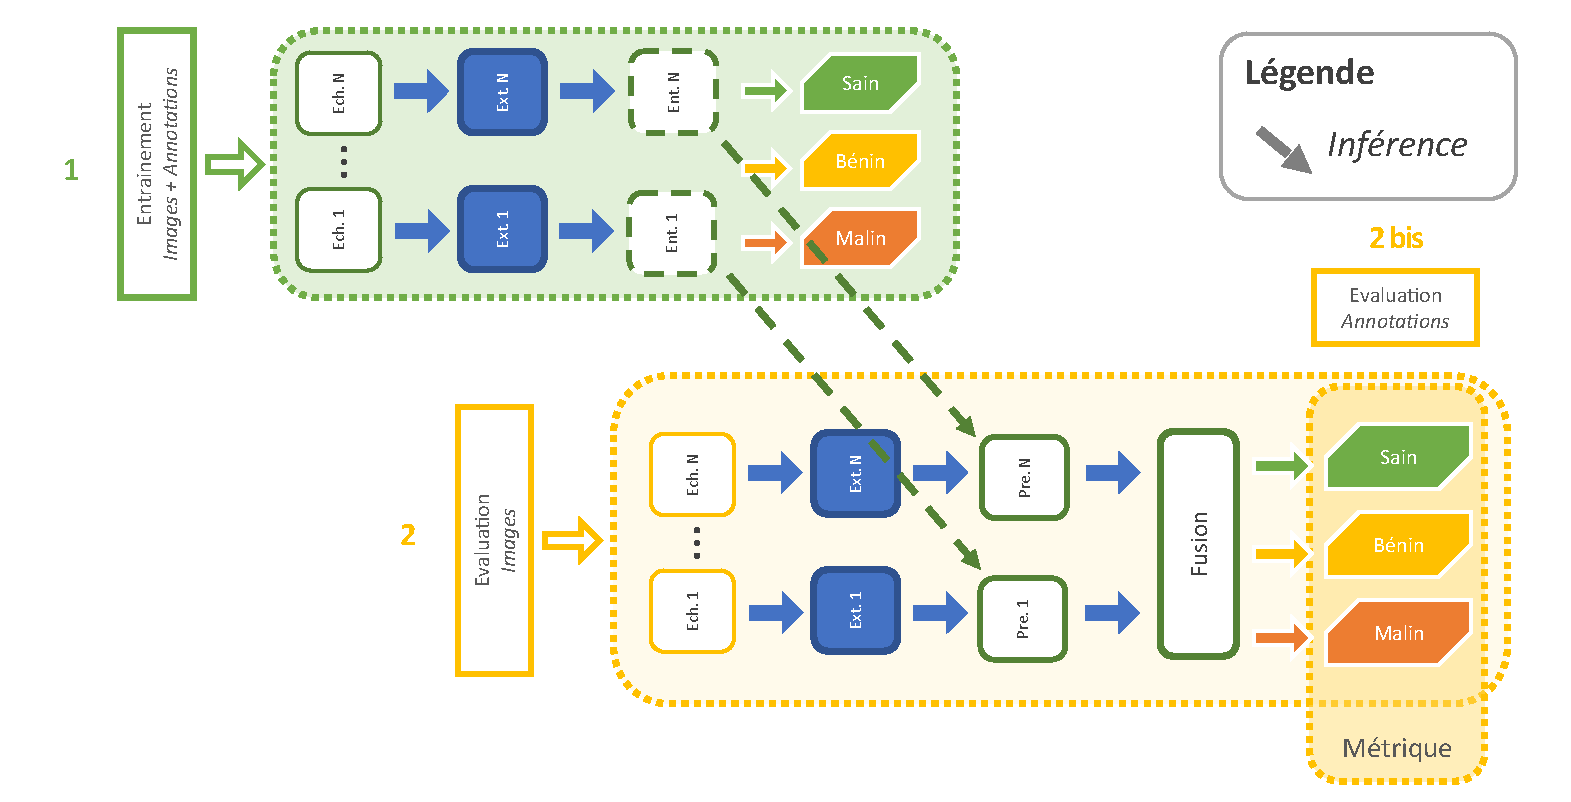
\includegraphics[width=0.85\linewidth]{contents/chapter_6/resources/scheme_image_improvement_multiscale_decision.pdf}
    \caption{Schéma de représentation du système multi-échelle, sur la base d'extractions et de prédictions à diverses échelles et par agrégation de ces décisions.}
    \label{fig:scheme_image_improvement_multiscale_decision}
\end{figure}\par

Ainsi, les diverses expériences de cette sous-section sont menées à l'aide des modes d'extraction précédemment étudiés dans le \Cref{chap:chapter_5}. Dans un premier temps, les descripteurs d'Haralick~\al{Haralick1973} sont employés et permettent l'extraction de 56 caractéristiques. Dans un second temps, le transfert de connaissances par l'utilisation de l'architecture de \gls{cnn} ResNet-50~\cite{He2016} pré-entraîné sur la base \textit{ImageNet}~\cite{Canziani2016} est employé et permet l'extraction de 2048 caractéristiques. Les expériences menées lors de cette sous-section sont recensées dans la \Cref{tab:parameters_spatial_transfer_multiscale_nb_features}.\par

\begin{table}[H]
    \centering
    \begin{tabular}{llll}
        \toprule
                                                    &           & \multicolumn{2}{l}{Nombre de caractéristiques}    \\ \hline
        \multirow{2}{*}{Fusion de caractéristiques} & Haralick  & \multicolumn{2}{l}{224 (56 $\times$ 4)}           \\ \cline{2-4}
                                                    & ResNet-50 & \multicolumn{2}{l}{8192 (2048 $\times$ 4)}        \\ \hline
        \multirow{2}{*}{Fusion de prédictions}      & Haralick  & 56 / échelle   & \multirow{2}{*}{\begin{tabular}[c]{@{}l@{}}4 (1 $\times$ 4) / Décisions\\ 12 (3 $\times$ 4) / Scores\end{tabular}} \\ \cline{2-3}
                                                    & ResNet-50 & 2048 / échelle &                                  \\
        \bottomrule
    \end{tabular}
    \caption{Listes des méthodes sur base de décomposition spatiale multi-échelle et leur nombre de caractéristiques extraites associées.}
    \label{tab:parameters_spatial_transfer_multiscale_nb_features}
\end{table}\par
\clearpage

\section{Approche par fenêtre glissante}
Lors de la section précédente, des schémas multi-échelle permettant une compréhension à divers niveaux ont été évoqués. Cette nouvelle section va s'orienter vers une compréhension des données à basse échelle, en partant de l'hypothèse qu'il existe un niveau de détail pour lequel les tissus peuvent être caractérisés avec suffisamment de précision.\par

Ce type d'approche est qualifié d'approche \textbf{par fenêtre glissante} ou par \textit{sliding window}. Néanmoins, le premier terme permet de visualiser le principe de fonctionnement consistant à balayer un espace de plus grande dimension par une fenêtre de dimension inférieure. Cette technique a permis des avancées pour diverses applications, dont~:~
\begin{itemize}
    \item la détection et localisation d'objets sur des images naturelles~\cite{Harzallah2009} ou encore la détection de cancer et de parties anatomiques sur images de radiologie~\cite{Helwan2017}, par motivation d'obtenir l'emplacement précis de certaines informations,
    \item la détection d'anomalies sur des images histologiques mais encore la classification de données conséquentes~\cite{Hou2016,Alqudah2019,Wei2019}, motivée par la contrainte matérielle impliquée par la taille de ces images ou par manque d'annotations.
\end{itemize}\par

Les données images de \gls{mcr} mises à la disposition de ce travail corroborent ce type de schéma, chacune d'entre elles contenant une composition de tissus divers. Ces labels au niveau de l'image répondent à une hiérarchie mise en place pour qualifier les relations entre ces tissus. Pour rappel, une annotation \textbf{maligne} qualifie une donnée comportant au minimum des tissus typiques d'une pathologie maligne mais peut également comporter des tissus bénins et sains~;~une annotation \textbf{bénigne} ne comporte que des tissus bénins ou potentiellement sains. Ces relations sont représentées sur la \Cref{fig:scheme_image_improvement_annotations_hierarchy}.\par

Ce travail se distingue de certains travaux~\cite{Hou2016,Alqudah2019} dans la mesure où il bénéficie d'une base de \textit{sous-images} d'une résolution spatiale \textbf{de 250 $\times$ 250 pixels}, annotées pour le besoin par l'un des spécialistes en dermatologie. Cette taille est un compromis entre le niveau de détail des types de tissus observables et les conclusions de Wiltgen~\al{Wiltgen2008}, suggérant une telle résolution. Néanmoins, afin de s'affranchir partiellement de l'influence de la taille de la fenêtre glissante, \textbf{une augmentation de ces sous-images à une résolution \textbf{de 500 $\times$ 500 pixels} par mosaïquage} est également employée.\par

\begin{table}[H]
    \centering
    \begin{tabular}{lll}
        \toprule
        \textbf{Modèle}                                 & \textbf{Hyperparamètres}  & \textbf{Valeurs}                          \\ \midrule
        \gls{svm} - Noyau linéaire                      & C                         & [0,001, 0,01, 0,1, 1, 10, 100, 1000]      \\ 
        \bottomrule 
    \end{tabular} 
    \caption{Table reprenant le modèle et les hyperparamètres du modèle de classification employé pour la détection à basse échelle des tissus dans le processus de fenêtre glissante.}
    \label{tab:parameters_image_improvement_sliding_window_models}
\end{table}\par

Dans le but de mettre en oeuvre le schéma de détection à basse échelle, les techniques d'extraction de caractéristiques jugées les plus pertinentes du \Cref{chap:chapter_5} sont utilisées, à savoir~:~
\begin{inlinerate}
    \item la méthode d'Haralick~\al{Haralick1973} comme représentante des méthodes spatiales,
    \item la méthode par décomposition en ondelettes de Daubechies comme représentante des méthodes fréquentielles,
    \item et enfin la méthode d'extraction par l'architecture ResNet-50 associée à une couche de Global Pooling - Moyenne comme représentante des méthodes par transfert de connaissances.
\end{inlinerate} Cette détection à basse échelle est réalisée à l'aide d'\textbf{une normalisation par Minimum / Maximum} associée à \textbf{un modèle \gls{svm} à noyau linéaire}, cette combinaison ayant été jugée la plus pertinente lors du \Cref{chap:chapter_5} et dont les paramètres sont listés dans la \Cref{tab:parameters_image_improvement_sliding_window_models}.\par

Afin de gérer les prédictions obtenues au niveau de la fenêtre glissante, plusieurs stratégies sont envisagées sur les décisions et les scores. Ainsi, plusieurs approches sont considérées, dont~:
\begin{itemize}
    \item   une approche au niveau des \textbf{décisions}, défini par l'ensemble $\mathbf{N}$. Cette approche aboutit à un vecteur de taille $1 \times n$ où $n$ correspond au nombre d'éléments extraits dans l'image. Deux méthodes ont été définies~:
            \begin{itemize}
                \item par \textbf{priorité}, dans laquelle est privilégiée la détection d'un élément d'une classe hiérarchiquement supérieure comme décision globale à l'image,
                \item par seuils \textbf{dynamiques}, dans laquelle sont déterminés des seuils optimaux d'éléments nécessaires à chaque classe pour décréter l'appartenance à l'une d'entre elles, et combinés à un système hiérarchique privilégiant les classes prioritaires.
            \end{itemize}
    \item   une approche au niveau des \textbf{scores}, défini par l'ensemble $\mathbf{R}$. Cette approche aboutit à un vecteur de taille $s \times n$ où $s$ correspond au nombre de scores de classes extrait et $n$ correspond au nombre d'éléments extraits dans l'image. Deux méthodes ont été définies, dont~:~
            \begin{itemize}
                \item par seuil \textbf{dynamique}, dans un premier temps cette méthode procède à une réduction de l'information à l'aide d'une fonction maximum, permettant de réduire celui-ci à vecteur de taille $1 \times s$ focalisé sur la confiance maximum en chaque classe. Dans un second temps, des seuils optimaux représentant la confiance minimale nécessaire sont déterminés sur ces scores, combinés là encore à un système hiérarchique privilégiant les classes prioritaires.
                \item par \textbf{classification}, le vecteur de scores est alors considéré comme un vecteur de caractéristiques fourni en entrée d'un modèle \gls{svm} linéaire, dont les hyperparamètres utilisés sont ceux de la \Cref{tab:parameters_image_improvement_sliding_window_models}.
            \end{itemize}
\end{itemize}\par

Dans ce travail, le scénario portant sur l'extraction de caractéristiques seules à l'aide de la fenêtre glissante, puis à la fusion de ces caractéristiques au niveau de l'image, n'est pas considéré. En effet, ce type de scénario génère bien trop de caractéristiques pour pouvoir être correctement traité au niveau de l'image. De plus, ce type de schéma perd l'une des motivations de cette méthode, à savoir isoler les parties d'images susceptibles de contenir les tissus d'intérêt.\par
 
Les paramètres propres à cette méthode sont visibles dans la \Cref{tab:parameters_image_improvement_sliding_window_parameters}. Afin de visualiser cette méthode, la \Cref{fig:scheme_image_improvement_sliding_features} met à disposition un schéma dans lequel ce processus est représenté.\par

\begin{table}[H]
    \centering
    \begin{tabular*}{0,6\linewidth}{l@{\extracolsep{\fill}}l}
        \toprule
        \textbf{Résolution spatiale}& \textbf{Chevauchement}\\ \hline
        250 $\times$ 250              & 0~\%                  \\ \hline
        250 $\times$ 250              & 25~\%                 \\ \hline
        250 $\times$ 250              & 50~\%                 \\ \hline 
        500 $\times$ 500              & 0~\%                  \\ \hline
        500 $\times$ 500              & 25~\%                 \\ \hline
        500 $\times$ 500              & 50~\%                 \\
        \bottomrule
    \end{tabular*}
    \caption{Ensemble des paramètres d'expérimentations menées par l'approche de type fenêtre glissante. L'étude de l'impact de la résolution spatiale est limitée aux valeurs de 250 $\times$ 250 et 500 $\times$ 500, mais également du chevauchement sur des valeurs de 0~\%, 25~\% et 50~\%.}
    \label{tab:parameters_image_improvement_sliding_window_parameters}
\end{table}\par

\begin{landscape}
\begin{figure}[H]
    \centering
    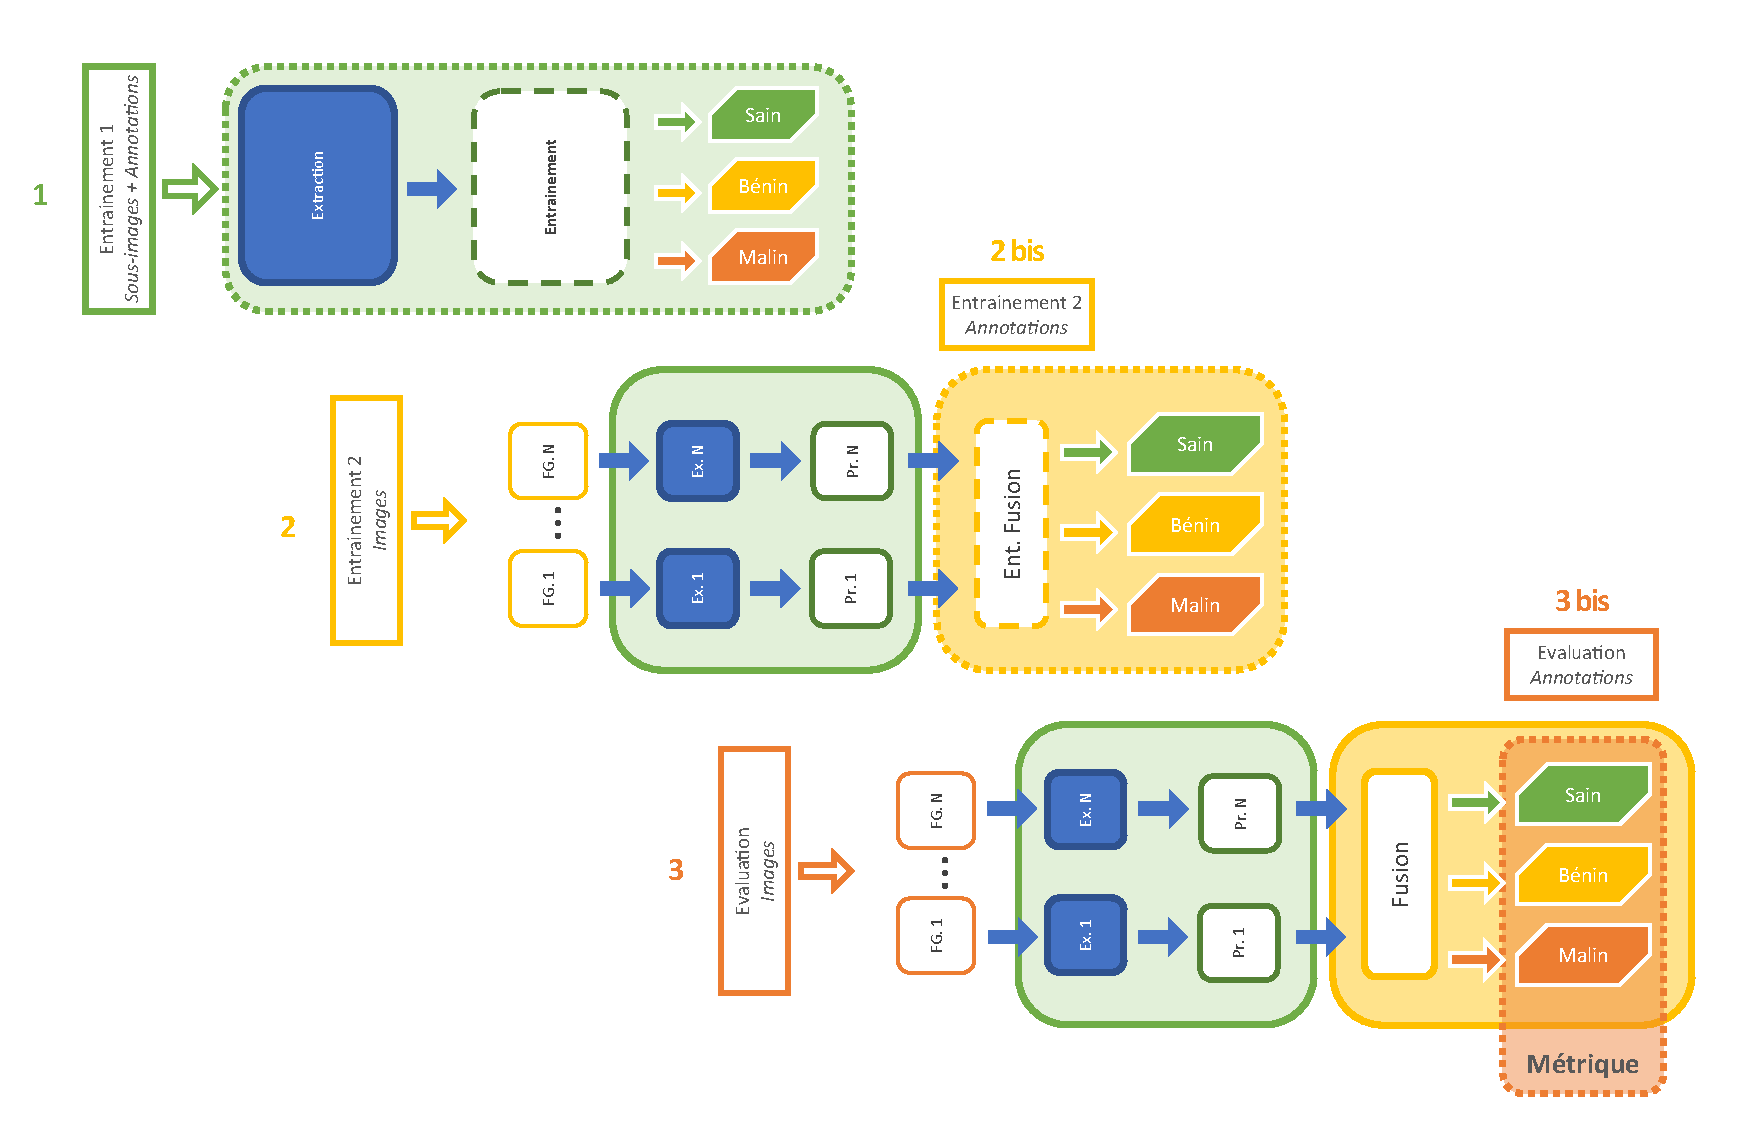
\includegraphics[width=0.8\linewidth]{contents/chapter_6/resources/scheme_image_improvement_sliding_features.pdf}
    \caption{Schéma de représentation du système de prédiction par fenêtre glissante. Ce schéma en deux temps propose de prédire sur une multitude de sous parties de l'image originale puis de fusionner les diverses prédictions afin de fournir une prédiction globale à l'image. Ainsi, une première phase d'entraînement est réalisée à l'aide des sous-images. Puis, le modèle entraîné permet de prédire au niveau des images par principe de fenêtre glissante pour lequel un second modèle permet de définir quels seuils sont critiques.}
    \label{fig:scheme_image_improvement_sliding_features}
\end{figure}\par
\end{landscape}

\section{Réglage fin de réseaux de convolution}
Dans cette partie, le réglage fin ou \textit{fine tuning} des \gls{cnn} est considéré sur cette problématique. En effet, ce principe est sollicité dans de nombreuses thématiques de recherche au moment de la rédaction de ce manuscrit, comme par exemple pour de la détection de plans d'intérêts sur des images par ultrasons~\cite{Chen2015}, mais aussi de plans cardiaques sur des images d'\gls{irm}~\cite{Margeta2015}. Également, ce principe est utilisé de manière très encourageante dans des applications visant à de la détection de pathologies sur des acquisitions de rayons X réalisées sur des seins~\cite{Lotter2017} ou encore sur des poumons~\cite{Gao2016}.\par

C'est de manière naturelle que cette section s'oriente en ce sens, en se consacrant à ses divers aspects à l'aide de sous-sections propres à chaque concept. Tout d'abord, une présentation du principe de réglage fin et des choix opérés est réalisée. Puis, les diverses techniques mises en œuvre pour tirer parti de ce principe sont présentées, dont~:
\begin{inlinerate}
    \item l'augmentation de données,
    \item et le programme d'apprentissage.
\end{inlinerate}\par

\subsection{Présentation et mise en oeuvre de la méthode}
Le réglage fin est une extension de l'apprentissage par transfert, dans lequel sont substituées les couches de classification initiales du réseau par de nouvelles couches adaptées au problème. Cette approche se distingue dans la mesure où tout ou partie du réseau est ré-entraîné à partir des poids existants~\cite{Tajbakhsh2016}. Ce mode d'apprentissage est utilisé lorsque les données propres au nouveau problème sont suffisantes, et permet à l'instar du simple apprentissage par transfert d'obtenir un réseau plus adapté au problème cible. Néanmoins, ce mode d'apprentissage \textbf{nécessite des ressources et un temps d'entraînement plus conséquent}.\par

Afin de procéder à ce réglage fin, il est nécessaire de déterminer une architecture cible permettant de gérer au mieux la complexité des données. Par exemple, un travail récent~\cite{Park2019} privilégie dans cette démarche l'utilisation d'une architecture \textit{ResNet-50}~\cite{He2016} pour la détection de lésions pulmonaires sur des images de rayons X et propose la localisation de ces dernières. Néanmoins, aucune justification ne semble avoir été apportée sur le choix de cette architecture, et aucune information n'est stipulée sur le type de \textit{Global Pooling} employé par ce travail.\par

Lors du \Cref{chap:chapter_5}, les résultats des architectures de \gls{cnn} pré-entraînés sur la base \textit{ImageNet} ont été comparés par application du principe de transfert de connaissances. Cette expérience a permis de déterminer de manière empirique la pertinence de l'\textbf{architecture de \gls{cnn} ResNet-50~\cite{He2016} associée à une couche de Global Pooling - Moyenne} sur cette problématique. Ainsi, ce travail suppose que l'architecture \textit{ResNet-50}~\cite{He2016} associée à une couche de \textit{Global Pooling - Moyenne} couplée au principe du réglage fin est en mesure de spécialiser le réseau à la problématique de lésion de la peau sur des images de \gls{mcr}, et d'améliorer \textit{in fine} ses performances.\par

Suivant ce constat, l'initialisation de cette architecture \textit{ResNet-50} est réalisée \textbf{à l'aide de poids issus d'un entraînement sur la base ImageNet}. Dans un premier temps, \textbf{la dernière couche totalement connectée de ce réseau sur base d'une activation \textit{softmax} est retirée}, prévue pour supporter les 1000 classes de la base de données \textit{ImageNet}. Dans un second temps, \textbf{une nouvelle couche totalement connectée de trois classes sur base d'une activation \textit{softmax} est ajoutée} afin de supporter les annotations saines, bénignes et malignes. Dans la mesure où ce travail tente de résoudre une problématique à plusieurs classes, \textbf{une fonction de coût de type entropie-croisée} est utilisée, suggérée par des travaux dont la problématique est équivalente~\cite{Barbu2016,Park2019}.\par

En termes de paramètres, la taille des lots ou \textit{batch size} \textbf{est réglée à une valeur de 8} pour des raisons de limitations matérielles. Néanmoins, une taille plus conséquente permet une meilleure stabilité de la convergence des \gls{cnn}. De plus, il est utile de préciser que l'ensemble des données de \gls{mcr} dédié à l'entraînement est utilisé lors de chacune de ces \textit{epochs}. Le nombre d'itérations ou \textit{epochs} n'est pas stipulé~;~\textbf{un critère d'arrêt en cas de convergence insuffisante après 5 itérations}, dont l'estimation est réalisée sur les données d'entraînement, est jugé suffisant dans ce contexte. Enfin, ce travail emploie une optimisation de type \textit{adam} tel que suggéré par de précédents travaux~\cite{Barbu2016,Park2019}, et dont \textbf{le taux d'apprentissage est réglé à une valeur de 0,001} faute de détails sur l'implémentation.\par

Pour finir sur ces aspects de mise en oeuvre, l'ensemble de ces éléments ont été réalisés à haut niveau à l'aide de la bibliothèque logicielle \textit{Keras}~\cite{chollet2015} en association à la bibliothèque de bas niveau \textit{Tensorflow}~\cite{Tensorflow2016}.\par

\subsection{Augmentation de données}
L'augmentation de données est une technique qui permet de corriger de manière artificielle le nombre d'exemples d'une base de données par application de transformations aux données d'origine~\cite{Wong2016,Taylor2018}. Cette technique est à ne pas confondre avec les méthodes de création d'échantillons virtuels à partir de l'espace des caractéristiques pour corriger les problèmes de balancements. L'augmentation de données, au sens de cette section, permet de corriger un non-balancement des annotations, mais est essentiellement employée dans le but d'enrichir le nombre d'exemples disponibles en contraignant le \gls{cnn} à se focaliser sur des éléments jugés essentiels à la résolution de la tâche visée.\par

Dans cette sous-section, cette technique est vue selon ces deux aspects mais surtout comme le moyen d'enrichir la base d'images de \gls{mcr} et ainsi d'éviter le sur-apprentissage potentiellement responsable de la dégradation des performances de prédiction. Les techniques considérées à cet effet correspondent à des transformations géométriques linéaires~\cite{Taylor2018}, opérées de manière aléatoire à chaque \textit{epochs} lors de l'entraînement. Bien évidemment, ces transformations ne sont appliquées que lors de l'entraînement, les images originales étant employées lors de l'évaluation. Les transformations considérées sont celles susceptibles de se produire dans un contexte clinique lors de l'acquisition des images, dont~:
\begin{inlinerate}
    \item la \textbf{rotation},
    \item la \textbf{translation},
    \item ou encore la \textbf{symétrie}.
\end{inlinerate} De plus, un repliement de l'information est réalisé pour combler le vide généré par ces opérations, jugé plus \textit{réaliste} sur les images traitées, que l'application d'une unique valeur de remplissage.\par

Ainsi, l'ensemble des paramètres de transformation utilisés lors de l'étape d'augmentation des données sont décrit dans la \Cref{tab:parameters_image_improvement_data_augmentation}. Cette étape s'appuie à cette fin sur le module d'augmentation de données de la bibliothèque logicielle \textit{Keras}~\cite{chollet2015}.\par

\begin{table}[H]
    \centering
    \begin{tabular}{ll}
        \toprule
        \textbf{Nom}                            & \textbf{Valeurs}      \\ \midrule
        Rotation (en degrés)                    & [0 à 45]              \\ 
        Translation Horizontale (en pourcentage)& [0 à 20]              \\ 
        Translation Verticale (en pourcentage)  & [0 à 20]              \\  
        Symétrie Horizontale                    & [Désactivée, Activée]  \\  
        Symétrie Verticale                      & [Désactivée, Activée]  \\ 
        \bottomrule 
    \end{tabular} 
    \caption{Table recensant les paramètres de transformation utilisés sur les données images de \gls{mcr} de manière aléatoire lors de l'entraînement.}
    \label{tab:parameters_image_improvement_data_augmentation}
\end{table}\par

\subsection{Programme d'apprentissage}
Le programme d'apprentissage ou \textit{Curriculum Learning} est une démarche visant par analogie à l'humain, à entraîner tout \gls{cnn} en proposant diverses tâches intermédiaires avec une difficulté croissante, afin d'accomplir avec une plus grande efficacité une tâche plus complexe. La raison technique derrière ce principe est de simplifier l'espace de recherche de la tâche cible, afin de trouver plus efficacement un minimum optimal au sein de la fonction de coût, comme suggéré par ses auteurs~\cite{Bengio2009}.\par

De récents travaux menés sur des images médicales, issue de rayons X, ont permis par cette approche d'augmenter les performance de détection de \gls{cnn} sur des cancers du sein~\cite{Lotter2017} ou encore des pathologies pulmonaires~\cite{Park2019}. La démarche suivie par ces deux travaux, est de procéder à l'extraction de sous images de taille restreinte autour des dites lésions avérées, en conservant la même propriété d'échelle que les images initiales. Cette extraction permet de réduire la résolution et la complexité du problème en proposant au réseau des images moins volumineuses et davantage focalisées sur des éléments clés afin d'éviter potentiellement des convergences non pertinentes. La gestion de données à échelles multiples sur \gls{cnn} ne donnant pas toujours lieu à des résultats suffisants~\cite{VanNoord2017}, une seconde étape d'entraînement est ensuite réalisée sur les images de taille réelle afin de former le réseau au problème définitif.\par

En complément de cette technique, la première phase de l'entraînement du \gls{cnn} est réalisée en deux temps. En effet, l'ajout de nouvelles couches connectées sous-entend une initialisation aléatoire de ces dernières. Ce phénomène peut conduire à une mauvaise optimisation de certains poids, provenant du caractère aléatoire de l'étape d'initialisation. Ainsi, une immobilisation des couches liées à l'extraction des caractéristiques est réalisée dans un premier temps (pré-entraînement), avant de procéder à l'entraînement du réseau dans sa totalité dans un second temps (entraînement). Ce processus d'entraînement en deux temps est schématisé sur la \Cref{fig:scheme_image_fine_tune}.\par

\begin{figure}[H]
    \centering
    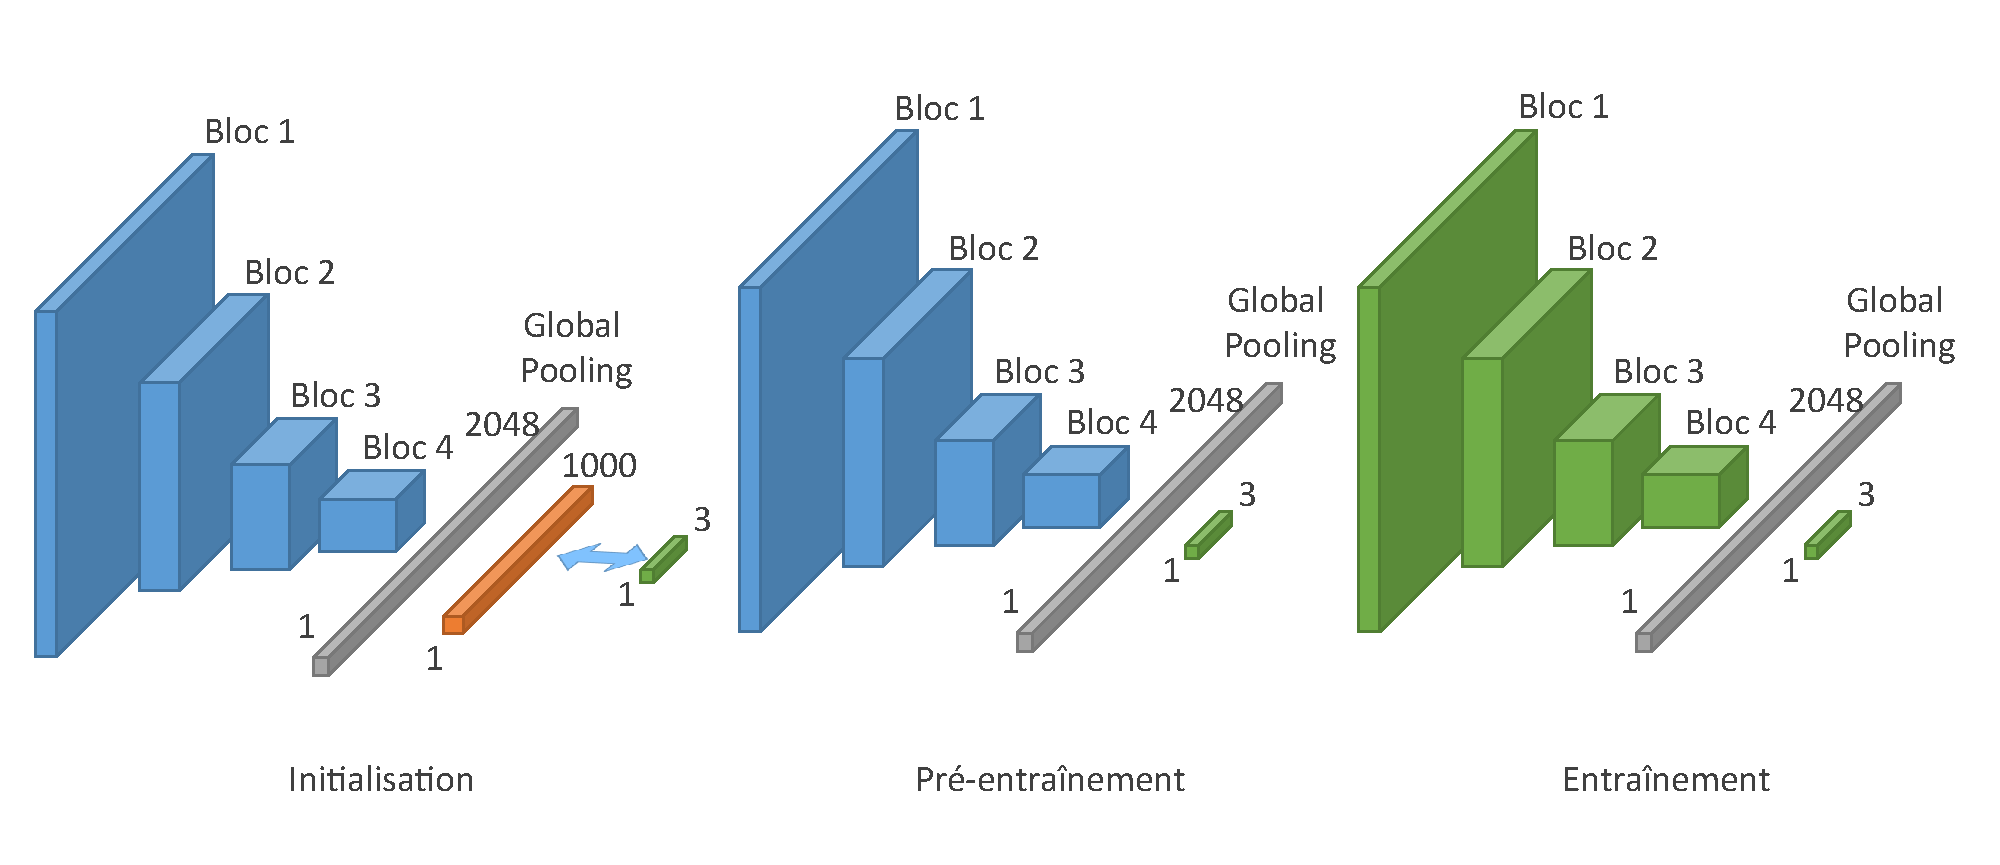
\includegraphics[width=\linewidth]{contents/chapter_6/resources/scheme_image_improvement_image_fine_tune.pdf}
    \caption{Schéma de représentation du processus de réglage fin utilisé dans ce travail. Celui-ci se décompose d'une étape d'initialisation dans le but de substituer les couches de classification, puis un pré-entraînement permet d'initialiser les poids avant de procéder à l'entraînement.}
    \label{fig:scheme_image_fine_tune}
\end{figure}\par
\clearpage

\section{Présentation des résultats}
Lors des précédentes sections ont été décrites les méthodes envisagées dans le but d'accroître la performance des prédictions au niveau des images de \gls{mcr} mais également leur compréhension. Par cette nouvelle section, les résultats obtenus par ces méthodes sont présentés. Dans une première sous-section, le protocole d'expérimentation suivi pour mesurer les performances de ces méthodes et l'organisation des résultats sont détaillés, puis dans une seconde sous-section, les résultats des diverses méthodes sont présentés.\par

\subsection{Protocole d'expérimentation}
Le protocole d'expérimentation suivi est similaire à celui du \Cref{chap:chapter_5}, afin que les résultats obtenus dans ce chapitre puissent être mis en parallèle et comparés avec ceux précédemment obtenus. Pour rappel, une \textbf{validation croisée imbriquée} est employée car les métriques extraites par ce processus sont plus objectives sur les performances du système évalué que des systèmes de validation croisée standards~\cite{Cawley2010}. De plus, cette structure de validation est plus robuste face au biais~\cite{Cawley2010} et démontrée empiriquement moins sensible au biais et à la variance lorsque des valeurs de $k$ sont comprises entre 5 et 10~\cite{James2013}. Pour des critères similaires à ceux du précédent chapitre, lié au grand nombre d'expérimentations, et de comparaison avec les précédents résultats, \textbf{une valeur $k$ de 4} est choisie.\par

En terme de métrique de validation et d'évaluation, les expérimentations de ce chapitre se basent sur le \textbf{\fscore{}} permettant de représenter les mesures de précision et de rappel au sein d'une même métrique binaire. Par ailleurs, cette métrique a été employée lors du \Cref{chap:chapter_5} et possède une bonne robustesse face à des déséquilibres de données. Concernant la présentation des résultats de l'évaluation, chaque méthode propose deux scores. D'une part, \textbf{un score pondéré} dont l'objectif est de fournir une indication de performance sur les trois classes. D'autre part, \textbf{un score malin} dont l'objectif est de renseigner sur la capacité d'une méthode à isoler particulièrement les données malignes.\par

D'un point de vue organisationnel, la prochaine sous-section propose un premier volet dédié aux résultats de classification des méthodes proposées, et met en évidence les combinaisons permettant la maximisation des scores ainsi que les résultats complets à l'aide de tables prévues à cet effet. Lors du premier paragraphe, les résultats des expérimentations menées \textbf{par multi-échelle} sont présentés. Puis dans un second et troisième paragraphe, les résultats obtenus \textbf{par principe de fenêtre glissante} sont présentés à \textbf{une résolution spatiale de 250 $\times$ 250 pixels puis de 500 $\times$ 500 pixels}. Pour finir, un quatrième paragraphe présente les résultats des expérimentations \textbf{de \gls{cnn} associés au principe de réglage fin}.\par

Pour finir, ce chapitre propose un second volet consacré à des techniques permettant d'aller au-delà du seul score de classification. Le premier de ces paragraphes propose une solution simple permettant d'observer localement les résultats obtenus par fenêtre glissante. Ainsi, la mise en place d'un code couleur sur les décisions et les scores de prédiction, superposé à l'image d'origine permet de visualiser les éléments déterminants lors de la prédiction. Puis, les paragraphes suivants apportent des pistes sur la visualisation de décisions issues de \gls{cnn} par utilisation du principe de \gls{cam}.\par
\clearpage

\subsection{Résultats des expérimentations}
Cette section suit paragraphe par paragraphe l'organisation énoncée et débute par les résultats issus de la famille de méthodes \textbf{par résolutions multiples}. Pour la catégorie \textbf{par ondelettes} et à l'aide de la \textbf{méthode de Wiltgen~\al{Wiltgen2008}}, un \fscore{} de 0,65 associé à un écart-type de 0,08 est obtenu à trois classes~;~un \fscore{} de 0,71 associé à un écart-type de 0,06 est obtenu sur la classe maligne. Pour la catégorie de méthodes \textbf{spatiale} et à l'aide de la \textbf{méthode de fusion de caractéristiques}, un \fscore{} de 0,63 associé à un écart-type de 0,06 est obtenu à trois classes~;~un \fscore{} de 0,67 associé à un écart-type de 0,07 est obtenu sur la classe maligne. Pour finir, la catégorie de méthodes par \textbf{transfert de connaissances} et à l'aide de la \textbf{méthode de fusion de caractéristiques}, un \fscore{} de 0,76 associé à un écart-type de 0,06 est obtenu à trois classes~;~un \fscore{} de 0,83 associé à un écart-type de 0,02 est obtenu sur la classe maligne. Les résultats de l'expérimentation menée sur la résolution multiple sont visibles dans la \Cref{tab:results_image_improvement_multiresolution}.\par

\begin{table}[H]
    \centering
    \begin{tabular}{llcc}
        \toprule
        Catégories                  & Méthodes                      & \Fscore{} - Pondéré     & \Fscore{} - Malin     \\ \midrule
        \multirow{3}{*}{Ondelettes} & Haar                          & 0,65 $\pm$ 0,08         & 0,70 $\pm$ 0,06         \\
                                    & Wiltgen~\cite{Wiltgen2008}    & \textbf{0,66 $\pm$ 0,06}& \textbf{0,71 $\pm$ 0,06}\\
                                    & Halimi~\cite{Halimi2017a}     & 0,38 $\pm$ 0,02         & 0,41 $\pm$ 0,04         \\ \midrule
        \multirow{5}{*}{Spatial}    & Fusion de caractéristiques    & \textbf{0,63 $\pm$ 0,06}& \textbf{0,67 $\pm$ 0,07}\\
                                    & Décisions - Maximum           & 0,60 $\pm$ 0,10         & 0,64 $\pm$ 0,08         \\
                                    & Scores - Moyenne + Maximum    & 0,60 $\pm$ 0,10         & 0,66 $\pm$ 0,07         \\
                                    & Scores - Maximum + Maximum    & 0,59 $\pm$ 0,10         & 0,65 $\pm$ 0,08         \\
                                    & Scores - \gls{svm} Linéaire   & 0,57 $\pm$ 0,10         & 0,65 $\pm$ 0,04         \\ \midrule \rowcolor[HTML]{E7E6E6}
        \multirow{5}{*}{Transfert}  & Fusion de caractéristiques    & \textbf{0,76 $\pm$ 0,06}& \textbf{0,83 $\pm$ 0,02}\\ 
                                    & Décisions - Maximum           & 0,69 $\pm$ 0,10         & 0,78 $\pm$ 0,05         \\
                                    & Scores - Moyenne + Maximum    & 0,69 $\pm$ 0,11         & 0,79 $\pm$ 0,06         \\
                                    & Scores - Maximum + Maximum    & 0,69 $\pm$ 0,11         & 0,79 $\pm$ 0,06         \\
                                    & Scores - \gls{svm} Linéaire   & 0,72 $\pm$ 0,04         & 0,79 $\pm$ 0,03         \\
        \bottomrule
    \end{tabular}
    \caption{Résultats issus du processus de classification basé sur les décompositions multi-échelle exprimées à l'aide du \fscore.}
    \vspace{-1em}
    \label{tab:results_image_improvement_multiresolution}
\end{table}

Ce second paragraphe présente les résultats obtenus à l'aide de l'approche \textbf{par fenêtre glissante}, à partir \textbf{d'une résolution spatiale de 250 $\times$ 250 pixels}. Les résultats sont maximisés par l'utilisation de \textbf{l'extraction par transfert de connaissance} sur la base de sous-images, pour laquelle un \fscore{} de 0,91 associé à un écart-type de 0,02 est obtenu à trois classes~;~un \fscore{} de 0,82 associé à un écart-type de 0,03 est obtenu sur la classe maligne. Par la catégorie de \textbf{méthodes spatiales} combinée à la méthode de \textbf{Décision - Dynamique} et \textbf{sans chevauchement} aboutissent à un \fscore{} de 0,62 associé à un écart-type de 0,02 pour trois classes~;~un \fscore{} de 0,68 associé à un écart-type de 0,05 est obtenu sur la classe maligne. Par la catégorie de \textbf{méthodes fréquentielles} combinée à la méthode de \textbf{Score - Classification} et \textbf{avec un chevauchement de 50~\%} aboutissent à un \fscore{} de 0,61 associé à un écart-type de 0,07 pour trois classes~;~un \fscore{} de 0,68 associé à un écart-type de 0,06 est obtenu sur la classe maligne. Pour finir, par la catégorie de \textbf{méthodes de transfert de connaissances} combinée à la méthode de \textbf{Score - Classification} et \textbf{avec un chevauchement de 50~\%} aboutissent à un \fscore{} de 0,78 associé à un écart-type de 0,03 pour trois classes~;~un \fscore{} de 0,82 associé à un écart-type de 0,02 est obtenu sur la classe maligne. Les résultats détaillés obtenus par principe de fenêtre glissante dont la résolution spatiale est de 250 $\times$ 250 pixels, sont présentés dans la \Cref{tab:results_image_improvement_sliding_window}.\par

\afterpage{\begin{landscape}
\begin{table}[p]
    \centering
    \begin{tabular}{lllcccccc}
		\toprule
		\multirow{2}{*}{Taille}     & \multirow{2}{*}{Chevauchement}& \multirow{2}{*}{Mode}     & \multicolumn{2}{c}{Spatial}                   & \multicolumn{2}{c}{Fréquence}                 & \multicolumn{2}{c}{Transfert}                 \\
		                            &                               &                           & Pondéré               & Malin                 & Pondéré               & Malin                 & Pondéré               & Malin                 \\ \midrule
		250                         & Aucune                        & Sous-images               & 0,67 $\pm$ 0,10         & 0,41 $\pm$ 0,13         & 0,72 $\pm$ 0,07         & 0,44 $\pm$ 0,10         & \textbf{0,91 $\pm$ 0,02}& \textbf{0,82 $\pm$ 0,03}\\ \midrule
		\multirow{12}{*}{250}       & \multirow{4}{*}{0~\%}          & Décision - Priorité       & 0,52 $\pm$ 0,02         & 0,67 $\pm$ 0,04         & 0,44 $\pm$ 0,06         & 0,65 $\pm$ 0,05         & 0,58 $\pm$ 0,04         & 0,71 $\pm$ 0,05         \\ 
							        &                               & Décision - Dynamique      & \textbf{0,62 $\pm$ 0,02}& \textbf{0,68 $\pm$ 0,05}& 0,57 $\pm$ 0,06         & 0,67 $\pm$ 0,04         & 0,75 $\pm$ 0,02         & 0,80 $\pm$ 0,03         \\
							        &                               & Score - Dynamique         & 0,54 $\pm$ 0,02         & 0,63 $\pm$ 0,04         & 0,50 $\pm$ 0,08         & 0,66 $\pm$ 0,05         & 0,70 $\pm$ 0,03         & 0,76 $\pm$ 0,02         \\
							        &                               & Score - Classification    & 0,60 $\pm$ 0,05         & 0,66 $\pm$ 0,04         & 0,59 $\pm$ 0,08         & 0,65 $\pm$ 0,07         & 0,78 $\pm$ 0,03         & 0,81 $\pm$ 0,03         \\ \cline{2-9}
							        & \multirow{4}{*}{25~\%}         & Décision - Priorité       & 0,49 $\pm$ 0,10         & 0,67 $\pm$ 0,10         & 0,41 $\pm$ 0,10         & 0,65 $\pm$ 0,10         & 0,53 $\pm$ 0,05         & 0,70 $\pm$ 0,09         \\
							        &                               & Décision - Dynamique      & 0,62 $\pm$ 0,07         & 0,68 $\pm$ 0,11         & 0,58 $\pm$ 0,08         & 0,66 $\pm$ 0,09         & 0,75 $\pm$ 0,03         & 0,80 $\pm$ 0,04         \\
							        &                               & Score - Dynamique         & 0,52 $\pm$ 0,03         & 0,59 $\pm$ 0,06         & 0,49 $\pm$ 0,08         & 0,66 $\pm$ 0,10         & 0,72 $\pm$ 0,04         & 0,78 $\pm$ 0,03         \\
							        &                               & Score - Classification    & 0,62 $\pm$ 0,06         & 0,71 $\pm$ 0,06         & 0,57 $\pm$ 0,10         & 0,66 $\pm$ 0,08         & 0,78 $\pm$ 0,03         & 0,81 $\pm$ 0,03         \\ \cline{2-9}
							        & \multirow{4}{*}{50~\%}         & Décision - Priorité       & 0,46 $\pm$ 0,11         & 0,66 $\pm$ 0,08         & 0,39 $\pm$ 0,12         & 0,64 $\pm$ 0,08         & 0,49 $\pm$ 0,10         & 0,68 $\pm$ 0,08         \\
							        &                               & Décision - Dynamique      & 0,62 $\pm$ 0,03         & 0,68 $\pm$ 0,07         & 0,59 $\pm$ 0,10         & 0,67 $\pm$ 0,08         & 0,75 $\pm$ 0,03         & 0,80 $\pm$ 0,03         \\
							        &                               & Score - Dynamique         & 0,52 $\pm$ 0,06         & 0,63 $\pm$ 0,07         & 0,49 $\pm$ 0,10         & 0,65 $\pm$ 0,07         & 0,72 $\pm$ 0,03         & 0,80 $\pm$ 0,01         \\ \rowcolor[HTML]{E7E6E6}
		                            &                               & Score - Classification    & 0,61 $\pm$ 0,08         & 0,69 $\pm$ 0,08         & \textbf{0,61 $\pm$ 0,07}& \textbf{0,68 $\pm$ 0,06}& \textbf{0,78 $\pm$ 0,03}& \textbf{0,82 $\pm$ 0,02}\\ \midrule
		500                         & Aucune                        & Sous-images               & 0,67 $\pm$ 0,08         & 0,40 $\pm$ 0,10         & 0,70 $\pm$ 0,06         & 0,50 $\pm$ 0,08         & \textbf{0,90 $\pm$ 0,02}& \textbf{0,80 $\pm$ 0,02}\\ \midrule
		\multirow{12}{*}{500}       & \multirow{4}{*}{0~\%}          & Décision - Priorité       & 0,58 $\pm$ 0,08         & 0,63 $\pm$ 0,05         & 0,23 $\pm$ 0,11         & 0,00 $\pm$ 0,00         & 0,74 $\pm$ 0,05         & 0,76 $\pm$ 0,05         \\
							        &                               & Décision - Dynamique      & 0,59 $\pm$ 0,04         & 0,63 $\pm$ 0,05         & 0,28 $\pm$ 0,05         & 0,63 $\pm$ 0,05         & 0,72 $\pm$ 0,05         & 0,76 $\pm$ 0,05         \\
							        &                               & Score - Dynamique         & 0,50 $\pm$ 0,05         & 0,56 $\pm$ 0,15         & 0,53 $\pm$ 0,08         & 0,66 $\pm$ 0,04         & 0,70 $\pm$ 0,03         & 0,78 $\pm$ 0,04         \\
							        &                               & Score - Classification    & 0,59 $\pm$ 0,08         & 0,67 $\pm$ 0,07         & 0,36 $\pm$ 0,04         & 0,55 $\pm$ 0,17         & 0,69 $\pm$ 0,13         & 0,74 $\pm$ 0,08         \\ \cline{2-9}
							        & \multirow{4}{*}{25~\%}         & Décision - Priorité       & 0,55 $\pm$ 0,08         & 0,64 $\pm$ 0,07         & 0,23 $\pm$ 0,11         & 0,00 $\pm$ 0,00         & 0,77 $\pm$ 0,05         & 0,80 $\pm$ 0,04         \\
							        &                               & Décision - Dynamique      & 0,55 $\pm$ 0,10         & 0,63 $\pm$ 0,05         & 0,28 $\pm$ 0,05         & 0,63 $\pm$ 0,05         & 0,76 $\pm$ 0,04         & 0,80 $\pm$ 0,04         \\
							        &                               & Score - Dynamique         & 0,53 $\pm$ 0,03         & 0,55 $\pm$ 0,09         & \textbf{0,55 $\pm$ 0,07}& \textbf{0,67 $\pm$ 0,05}& 0,73 $\pm$ 0,03         & 0,80 $\pm$ 0,04         \\
							        &                               & Score - Classification    & 0,58 $\pm$ 0,07         & \textbf{0,67 $\pm$ 0,06}& 0,37 $\pm$ 0,04         & 0,55 $\pm$ 0,18         & 0,77 $\pm$ 0,05         & 0,81 $\pm$ 0,04         \\ \cline{2-9}
							        & \multirow{4}{*}{50~\%}         & Décision - Priorité       & 0,57 $\pm$ 0,08         & 0,67 $\pm$ 0,11         & 0,23 $\pm$ 0,07         & 0,00 $\pm$ 0,00         & 0,77 $\pm$ 0,03         & 0,81 $\pm$ 0,05         \\
							        &                               & Décision - Dynamique      & 0,58 $\pm$ 0,07         & 0,67 $\pm$ 0,11         & 0,28 $\pm$ 0,12         & 0,63 $\pm$ 0,12         & 0,76 $\pm$ 0,03         & 0,80 $\pm$ 0,05         \\
							        &                               & Score - Dynamique         & 0,52 $\pm$ 0,05         & 0,55 $\pm$ 0,06         & 0,55 $\pm$ 0,08         & 0,67 $\pm$ 0,13         & 0,73 $\pm$ 0,04         & 0,80 $\pm$ 0,05         \\ \rowcolor[HTML]{E7E6E6}
		                            &                               & Score - Classification    & \textbf{0,60 $\pm$ 0,06}& 0,65 $\pm$ 0,09         & 0,34 $\pm$ 0,05         & 0,39 $\pm$ 0,23         & \textbf{0,78 $\pm$ 0,02}& \textbf{0,81 $\pm$ 0,04}\\
		\bottomrule
    \end{tabular}
    \caption{Résultats issus du processus de classification basé sur le principe de fenêtre glissante exprimé à l'aide du \fscore. La première partie de ce tableau reprend les résultats obtenus à l'aide d'une fenêtre glissante de taille de 250 $\times$ 250 pixels tandis que la seconde partie se concentre sur les résultats d'une fenêtre glissante de taille de 500 $\times$ 500 pixels.}
    \label{tab:results_image_improvement_sliding_window}
\end{table}
\end{landscape}}

Afin de terminer sur cette approche \textbf{par fenêtre glissante}, ce paragraphe décrit les résultats obtenus à l'aide \textbf{d'une résolution spatiale de 500 $\times$ 500 pixels}. À nouveau, ces résultats sont maximisés par l'utilisation de \textbf{l'extraction par transfert de connaissance} sur la base de sous-images, pour laquelle un \fscore{} de 0,90 associé à un écart-type de 0,02 est obtenu à trois classes~;~un \fscore{} de 0,80 associé à un écart-type de 0,02 est obtenu sur la classe maligne. Pour la catégorie de \textbf{méthodes spatiales} combinée à la méthode de \textbf{Score - Classification} et \textbf{avec chevauchement de 50~\%}, un \fscore{} de 0,60 associé à un écart-type de 0,06 est obtenu à trois classes~;~le chevauchement doit être à une valeur de 25~\% pour permettre d'obtenir un \fscore{} de 0,67 associé à un écart-type de 0,06 est obtenu sur la classe maligne. Pour la catégorie de \textbf{méthodes fréquentielles} combinée à la méthode de \textbf{Score - Dynamique} et \textbf{avec un chevauchement de 25~\%}, un \fscore{} de 0,55 associé à un écart-type de 0,07 est obtenu à trois classes~;~un \fscore{} de 0,67 associé à un écart-type de 0,05 est obtenu sur la classe maligne. Pour finir, la catégorie de \textbf{méthodes de transfert de connaissances} combinée à la méthode de \textbf{Score - Classification} et \textbf{avec un chevauchement de 50~\%}, un \fscore{} de 0,78 associé à un écart-type de 0,02 est obtenu à trois classes~;~un \fscore{} de 0,81 associé à un écart-type de 0,04 est obtenu sur la classe maligne. Ces résultats sont détaillés dans la \Cref{tab:results_image_improvement_sliding_window}.\par

Ce nouveau paragraphe clôture à proprement parler les résultats de classification, en énonçant ceux issus des \gls{cnn}. Dans un premier temps, le \textbf{processus de réglage fin seul} est évalué afin de mesurer ses performances dans le cadre de son utilisation sur l'architecture \textbf{ResNet-50}. Par l'utilisation d'une couche de \textbf{Global Pooling - Moyenne}, un \fscore{} de 0,56 associé à un écart-type de 0,05 est obtenu à trois classes~;~un \fscore{} de 0,78 associé à un écart-type de 0,05 est obtenu sur la classe maligne. Dans un second temps, le \textbf{processus de réglage fin couplé au programme d'apprentissage} est évalué afin de mesurer l'influence de celui-ci. Par l'utilisation de l'architecture \textbf{ResNet-50 couplée à une couche de Global Pooling - Moyenne}, un \fscore{} de 0,51 associé à un écart-type de 0,07 est obtenu à trois classes~;~un \fscore{} de 0,67 associé à un écart-type de 0,05 est obtenu sur la classe maligne. L'ensemble de ces résultats de classification par réglage fin est disponible dans la \Cref{tab:parameters_image_improvement_fine}.\par

\begin{table}[H]
    \centering
    \begin{tabular}{llcc}
        \toprule
        Catégorie                               & Global Pooling                    & \Fscore{} - Pondéré                           & \Fscore{} - Malin                             \\ \midrule
        \multirow{2}{*}{Réglage fin}            & Maximum                           & 0,44 $\pm$ 0,05                                 & 0,69 $\pm$ 0,06                                 \\ \cline{2-4}
                                                & \cellcolor[HTML]{E7E6E6}Moyenne   & \cellcolor[HTML]{E7E6E6}\textbf{0,56 $\pm$ 0,05}& \cellcolor[HTML]{E7E6E6}\textbf{0,78 $\pm$ 0,05}\\ \midrule
        Programme d'apprentissage               & Moyenne                           & 0,51 $\pm$ 0,07                                 & 0,67 $\pm$ 0,05                                 \\
        \bottomrule
    \end{tabular}
    
    \caption{Résultats issus du processus de classification basé sur les \gls{cnn} par réglage fin et programme d'apprentissage exprimés à l'aide du \fscore.}
    \label{tab:parameters_image_improvement_fine}
\end{table}
\clearpage

\subsection{Méthodes de visualisation}
Enfin, cette section dédiée aux résultats se termine par la proposition d'extensions aux principes de fenêtre glissante et de réglage fin de \gls{cnn}. En effet, ces deux méthodes possèdent par leur nature, la capacité de localiser précisément l'origine d'une information. Dans le cadre de l'approche par fenêtre glissante, c'est de manière directe que ce principe permet de remonter à l'emplacement d'une décision. Deux modes de visualisation sont ainsi proposés, l'un basé \textbf{sur les décisions} en utilisant un code couleur propre à chacune des classes mais également \textbf{sur les scores} en utilisant le principe de code couleur précédent combiné à l'intensité de la transparence comme indicateur de confiance de la prédiction. Une taille de fenêtre glissante la plus fine permettra par cette technique d'obtenir une information visuelle de meilleure qualité, dualité qu'il est possible d'observer entre les résolutions spatiales de fenêtre glissante de 250 $\times$ 250 et 500 $\times$ 500. Des exemples de ces deux propositions de techniques de visualisation sont fournis via la \Cref{fig:exemple_image_improvement_well}.\par

\begin{figure}[H]
    \centering
    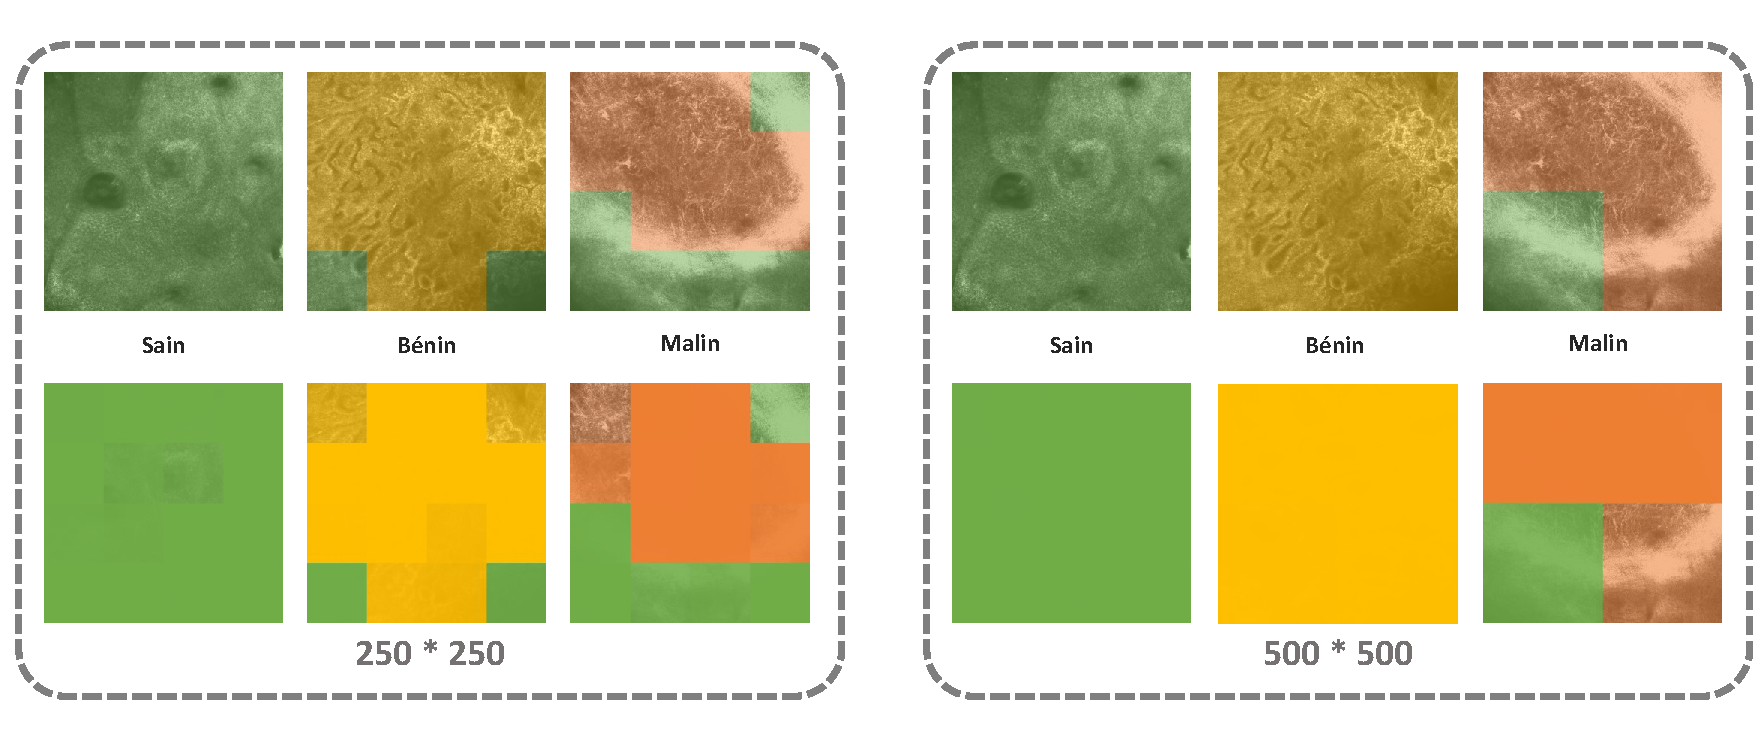
\includegraphics[width=\linewidth]{contents/chapter_6/resources/exemple_image_improvement_well.pdf}
    \caption{Exemple d'images correctement classifiées à l'aide du principe de fenêtre glissante. À gauche, résultats issus d'une fenêtre de classification de 250 par 250 pixels~;~À droite, résultats issus d'une fenêtre de classification de 500 par 500 pixels. En haut, représentations des décisions par code couleur : zones saines en vert, zones bénignes en jaune et zones malignes en orange~;~En bas, représentations des scores par les codes couleur précédents et intensités de transparence variables : zones de forte confiance en opaque et zones de faible confiance en translucide.}
    \label{fig:exemple_image_improvement_well}
\end{figure}\par

Le dernier principe de visualisation proposé dans cette sous-section dédiée aux résultats, se base sur les \gls{cnn} en exploitant le principe même de la convolution utilisée au sein de ces réseaux. De nombreux travaux se sont portés sur la compréhension des décisions issues de \gls{cnn} avec \textbf{la mise en évidence des filtres auto-déterminés de convolution}~\cite{Zeiler2014} ou encore la mise en lumière des zones responsables de l'activation d'une classe par le principe des \acrlong{cam}~\cite{Zhou2015}. La nouvelle méthode proposée dans cette sous-section exploite ce second principe de \gls{cam}, dont le fonctionnement est présenté sur le schéma de la \Cref{fig:scheme_image_improvement_cam}. Cette méthode consiste à pondérer le résultat de la dernière couche convolutive par les poids issus de la décision d'une classe. Ces recherches sur les \gls{cam} ont abouti à divers travaux de détections sur images naturelles dont résultent YOLO~\cite{Redmon2016} ou encore SSD~\cite{Liu2016}. Ainsi, diverses applications ont vu le jour sur de l'imagerie médicale afin de fournir une visualisation~\cite{jia2017} mais également des zones clés de diagnostic~\cite{Park2019}.\par 
\clearpage

Dans le dernier aspect de ce travail, la méthode des \gls{cam} est combinée à l'application d'un seuil sur ces valeurs, permettant de définir un masque de segmentation de la zone d'intérêt. Le seuil a été défini de manière arbitraire à une valeur de 85~\% du rang entre les valeurs minimum et maximum issues des \gls{cam}, permettant l'obtention des diverses segmentations présentées sur la \Cref{fig:example_image_improvement_ft}. Sur cette figure, sont représentés des exemples de tissus malins correctement détectés par la méthode, mais également non pertinents sur la partie basse de cette même figure. Ces exemples non pertinents nombreux peuvent s'expliquer par la faible performance obtenue sur l'entraînement des \gls{cnn}. Néanmoins, les intérêts de cette méthode sont multiples, puisque le principe de \gls{cam} permet par le seul passage d'une image de revenir aux zones d'activations à partir d'une tâche initiale de classification. De plus, cette méthode ne dépend pas de paramètres tel que la taille ou le chevauchement comme cela peut être le cas pour le principe de fenêtre glissante.\par

\begin{figure}[H]
    \centering
    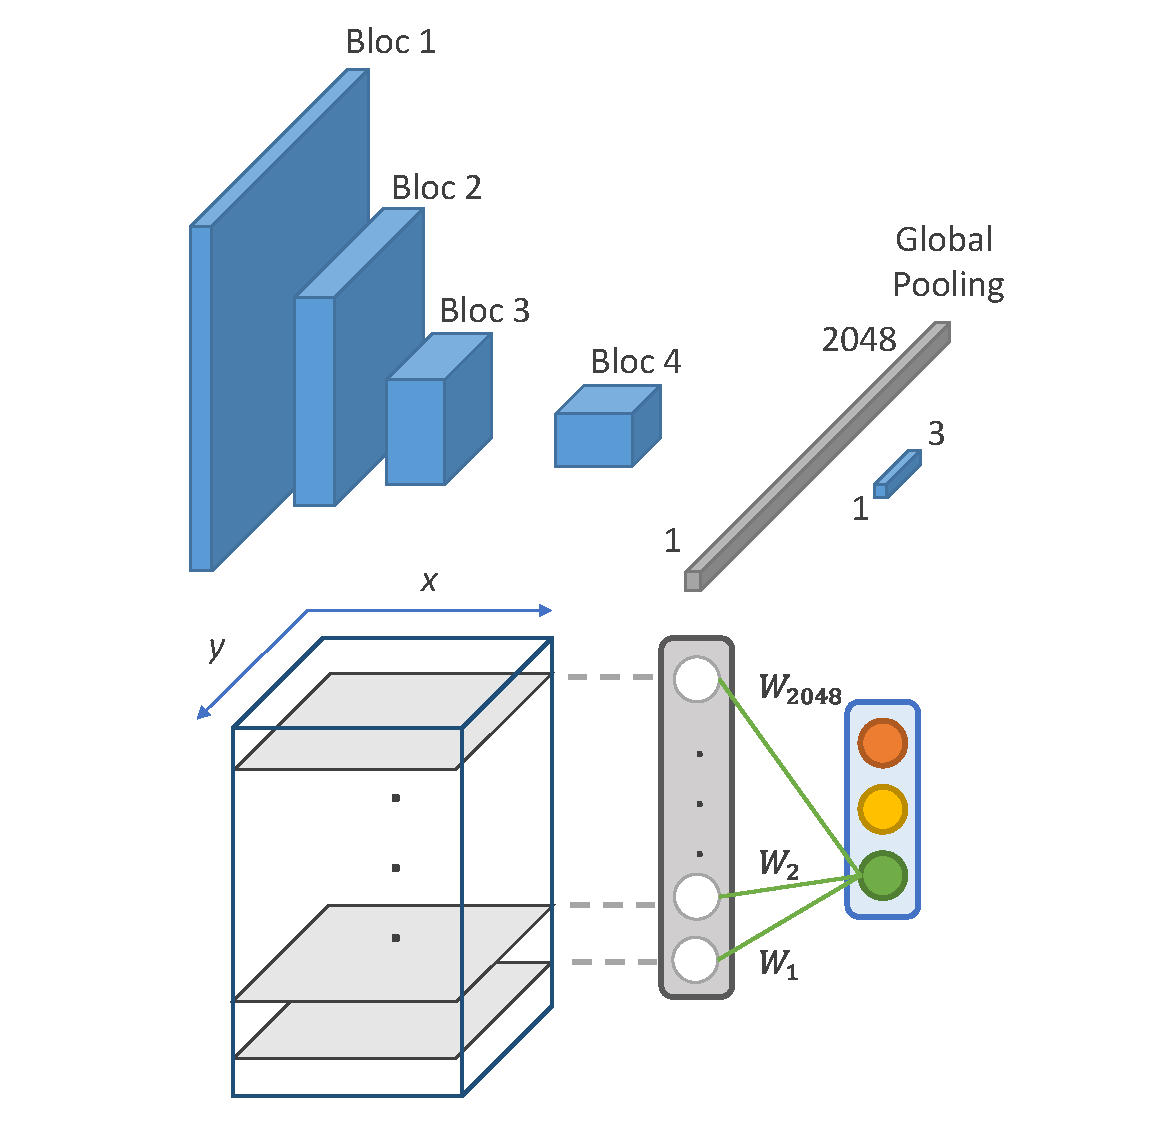
\includegraphics[width=\linewidth]{contents/chapter_6/resources/scheme_image_improvement_cam.pdf}
    \caption{Schéma d'explication du principe de \gls{cam} employé à but de segmentation des images de \gls{mcr}. Le réseau est entraîné sur la problématique cible, puis \textit{la ou les couches} de classification sont mobilisées dans le but d'obtenir les zones responsables de la décision par pondération des poids de chaque noeud de la classe considérée.}
    \label{fig:scheme_image_improvement_cam}
\end{figure}\par

\begin{figure}[p]
    \centering
    \begin{subfigure}{.48\textwidth}
      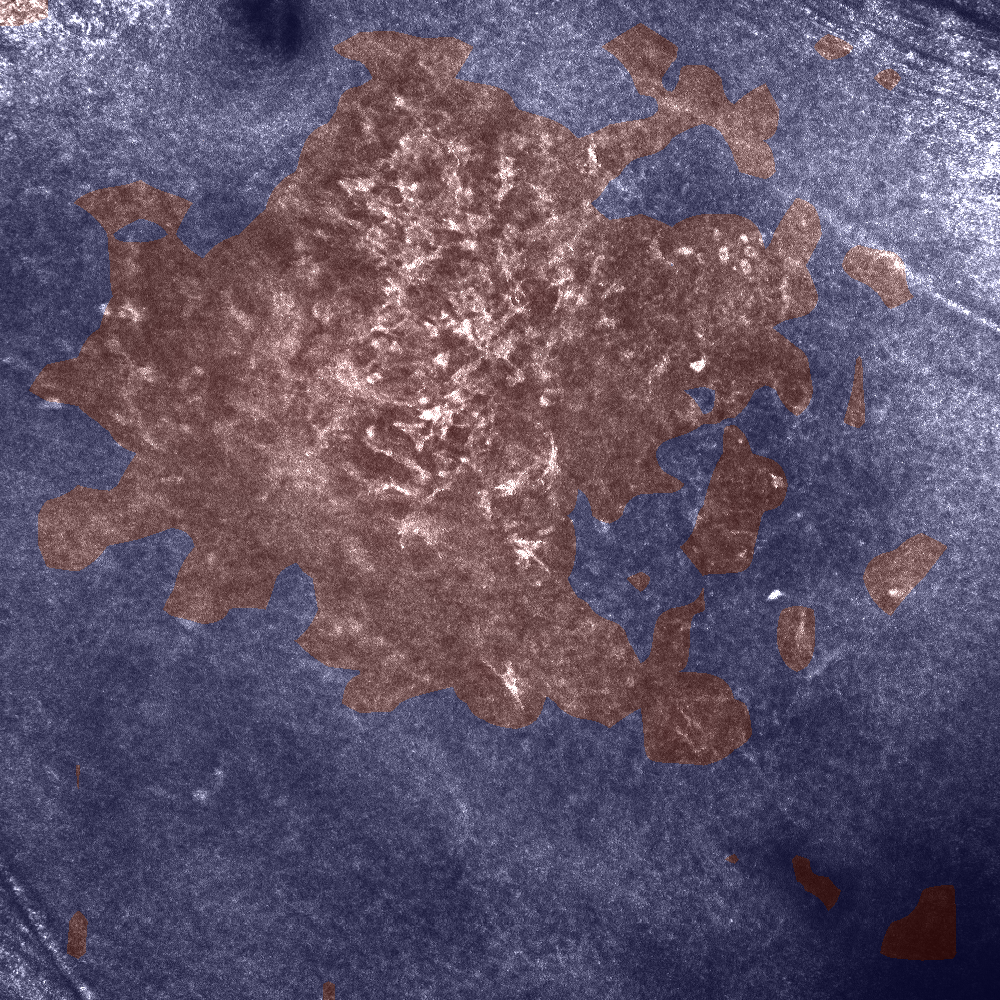
\includegraphics[width=\textwidth]{contents/chapter_6/resources/example_image_improvement_ft_well_1.png}
    \end{subfigure}
    \begin{subfigure}{.48\textwidth}
      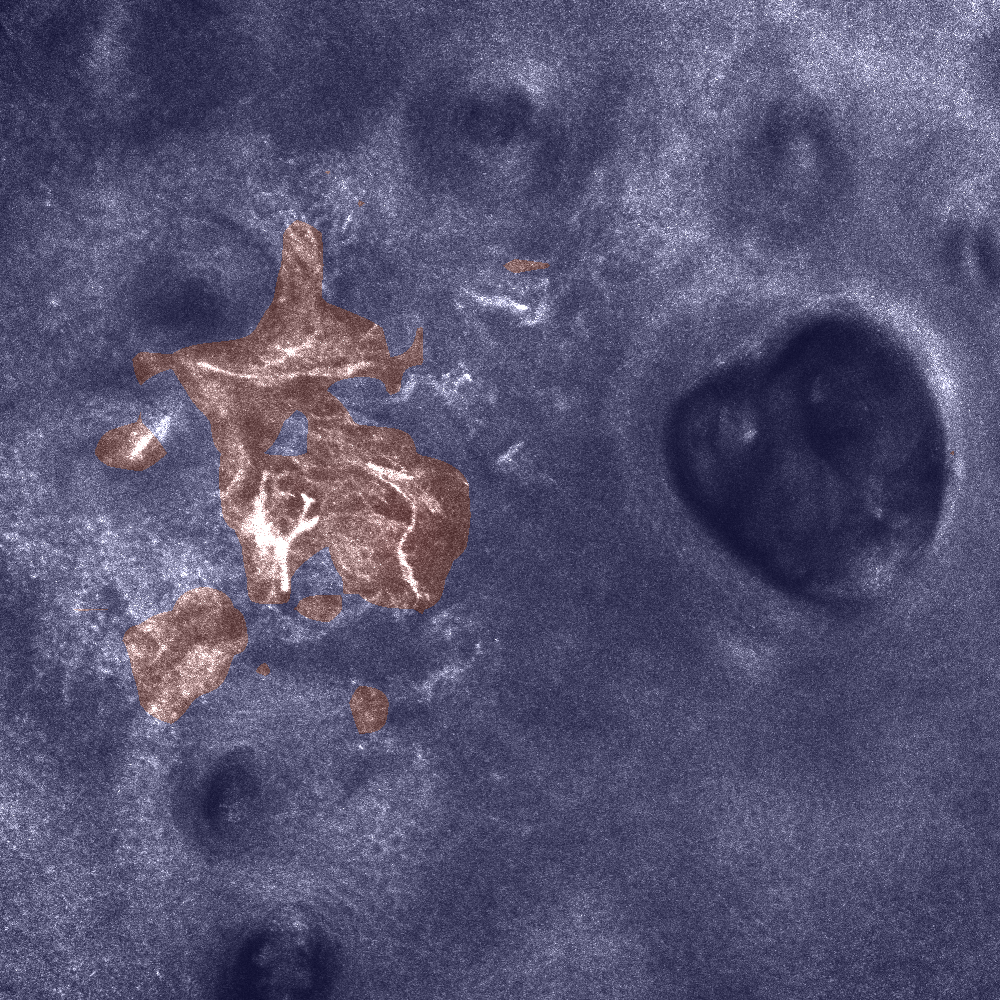
\includegraphics[width=\textwidth]{contents/chapter_6/resources/example_image_improvement_ft_well_2.png}
    \end{subfigure}
    
    \begin{subfigure}{.48\textwidth}
      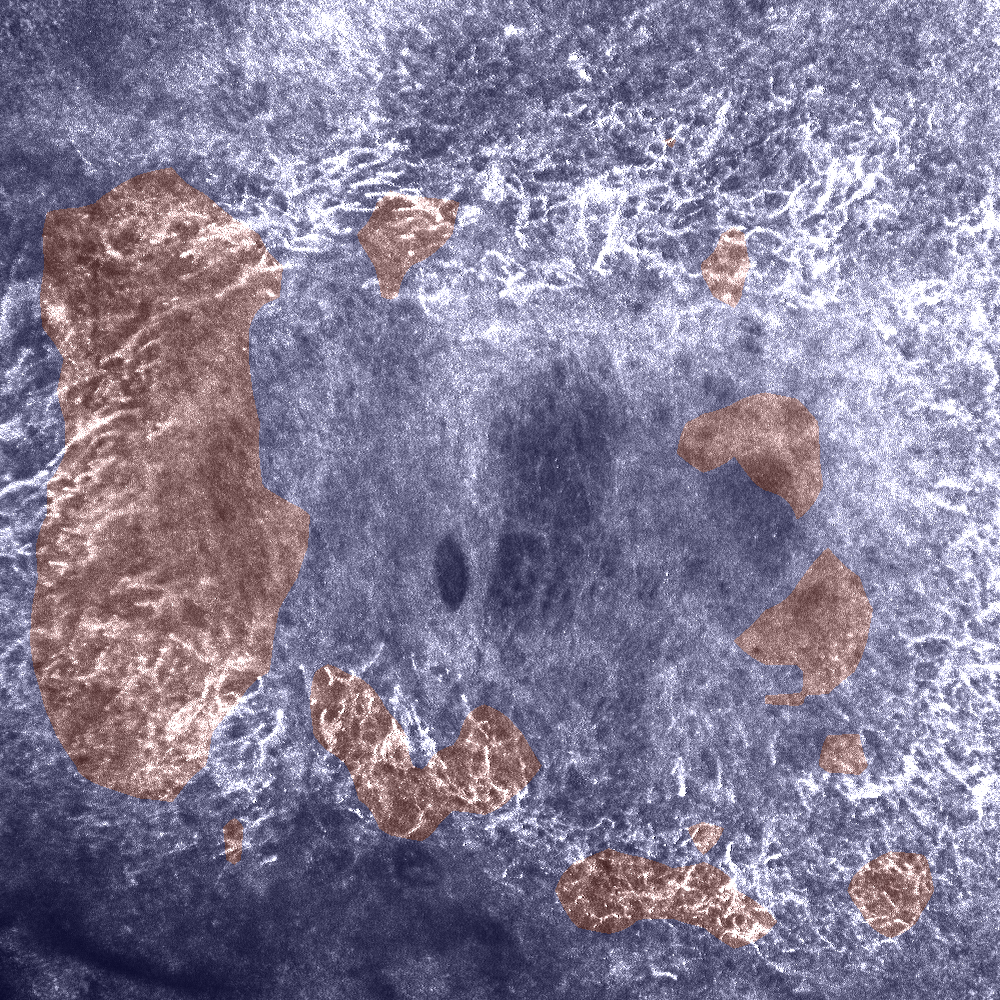
\includegraphics[width=\textwidth]{contents/chapter_6/resources/example_image_improvement_ft_misclassified_1.png}
    \end{subfigure}
    \begin{subfigure}{.48\textwidth}
      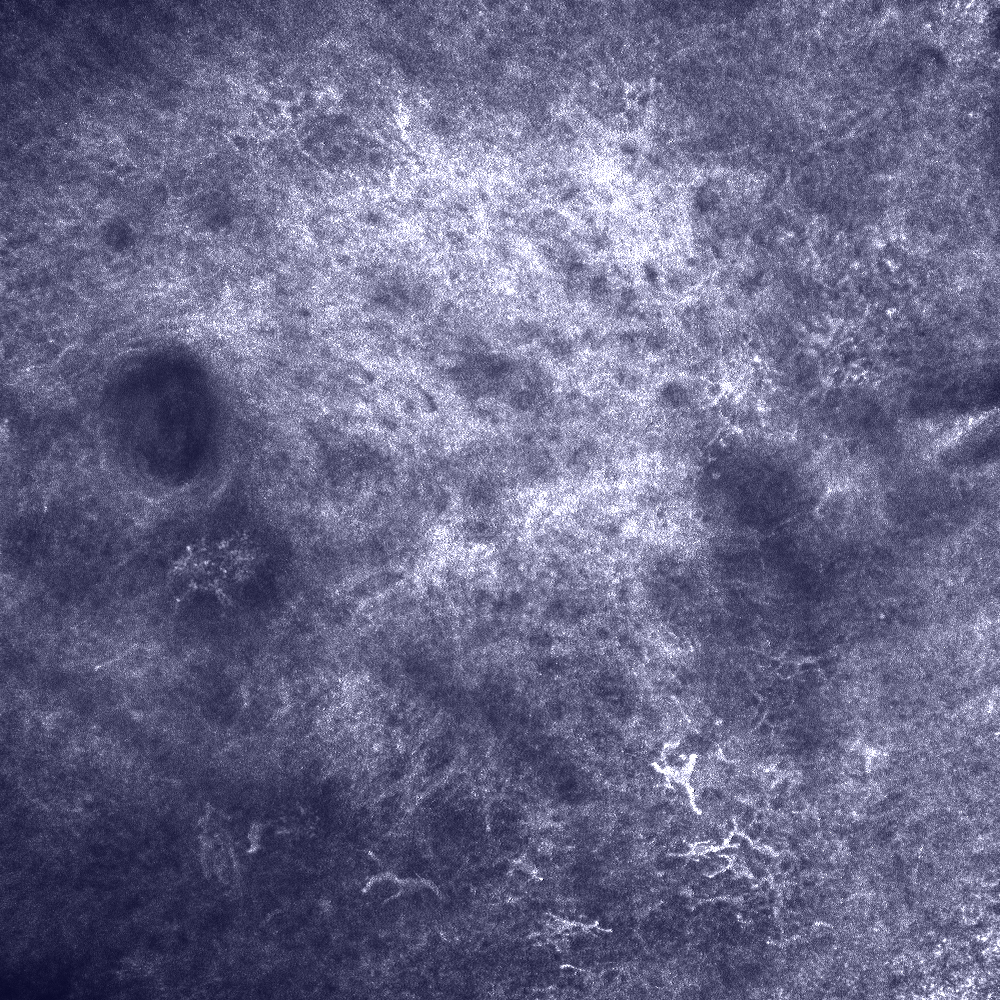
\includegraphics[width=\textwidth]{contents/chapter_6/resources/example_image_improvement_ft_misclassified_2.png}
    \end{subfigure}
    
    \caption{Exemples de l'extraction de zones d'activations par principe de \gls{cam}, avec application d'un seuil arbitraire à 85~\% entre la valeur minimum et maximum. En haut, exemples d'images malignes correctement gérées par ce principe~;~En bas, exemples d'images malignes partiellement segmentées ou incorrectement gérées par ce principe.}
    \label{fig:example_image_improvement_ft}
\end{figure}\par
\clearpage

\section{Discussion}
En premier lieu, les résultats issus de la décomposition en ondelettes multi-échelle sont sensiblement identiques à ceux présentés lors du \Cref{chap:chapter_5} à trois classes. Une amélioration significative des performances sur la détection d'éléments malins est à noter par la méthode en ondelettes de Wiltgen~\al{Wiltgen2008}, permettant l'obtention d'un \fscore{} de 0,71 $\pm$ 0,06, initialement à 0,68 $\pm$ 0,03. L'utilisation de l'ondelette mère de Haar par cette technique ne dégrade que très peu les résultats à deux et trois classes. En revanche, l'évaluation de la méthode proposée par Halimi~\al{Halimi2017a} aboutie à des performances proches de prédictions aléatoires sur les données de \gls{mcr} exploitées dans ce manuscrit. Des diverses méthodes proposées pour l'utilisation de caractéristiques spatiales et par transfert de connaissances, seule la fusion de caractéristiques s'est réellement avérée fonctionnelle. Cette technique a recueilli par l'utilisation du transfert de connaissances un \fscore{} de 0,76 $\pm$ 0,06 à trois classes et de 0,83 $\pm$ 0,02 pour la détection d'éléments malins.\par

En second lieu, une approche par fenêtre glissante a été employée afin d'améliorer la qualité des résultats. Par cette approche, la classification à trois classes obtenue par les diverses techniques d'extraction n'a pas ou peu été améliorée. Sur la détection d'éléments malins, seule la technique employant les descripteurs proposés par Haralick semble avoir recueilli de meilleurs résultats, voyant passer ceux-ci de valeurs de \fscore{} 0,68 $\pm$ 0,03 à 0,71 $\pm$ 0,06. D'une part, des deux méthodes employant un principe de prédiction sur les décisions, la proposition de méthode sur la base de seuil dynamique semble, comme espéré, la plus judicieuse, mais risque de délaisser certains cas cliniques selon la tolérance de ce seuil. D'autre part, des deux méthodes employant un principe de prédiction sur les scores, la proposition de méthode utilisant un modèle \gls{svm} linéaire semble la plus adaptée. Néanmoins, cette méthode risque de favoriser par une pondération plus grande certaines positions de la fenêtre glissante, tandis que la méthode sur seuil dynamique est invariante à cette position. Concernant les hypothèses de la fenêtre glissante, l'une d'entre elles avait été formulée sur le rôle important de la taille de fenêtre dans cette approche, et la tendance des résultats semble meilleure à l'aide d’une fenêtre de taille restreinte de 250 $\times$ 250 mais ces résultats ne sont pas significatifs. Une autre hypothèse supposait l'importance d'un chevauchement des acquisitions en provenance de la fenêtre glissante, et également la tendance des résultats semble plus optimiste sans chevauchement, cependant là encore ces résultats ne sont pas significatifs. Les résultats de cette expérience sont maximisés par l'utilisation de transfert de connaissances avec l'architecture ResNet-50, dans le cadre d'un chevauchement de 50~\% mais là encore les résultats ne sont pas suffisamment significatifs pour affirmer l'utilité de ce chevauchement. En addition, ce travail montre qu'il est possible de revenir assez facilement aux décisions à basse échelle par l'utilisation d'un code de couleur ou par opacité. Ce type d'approche pourrait permettre d'expliquer les décisions du système prédicatif et d'aiguiller ou de guider le spécialiste à focaliser son attention sur les zones les plus importantes. Il convient néanmoins de solutionner les performances de prédiction de ce système.\par 

Enfin, cette discussion se termine par l'étude des résultats liés au réglage fin dont les expériences ont été réalisées en deux temps, avec un simple réglage fin puis grâce la réalisation d'un programme d'apprentissage à l'aide des sous-images à disposition de ce travail. Par ces méthodes, les résultats ont été fortement impactés dans les deux cas, avec un \fscore{} par transfert de connaissances sur ResNet-50 initial de 0,77 $\pm$ 0,04 à trois classes et 0,82 $\pm$ 0,02 à deux classes~:~par réglage fin ces résultats descendent à des valeurs de 0,78 $\pm$ 0,05 à trois classes et 0,56 $\pm$ 0,05 à deux classes~;~par programme d'apprentissage ces valeurs ne sont plus que de 0,51 $\pm$ 0,07 à trois classes et 0,67 $\pm$ 0,05. Un fort sur-apprentissage de ce réseau est supposé malgré le mécanisme d'augmentation de données mis en place. En effet, les diverses phases d'apprentissage réalisées ont abouti à un \fscore{} compris entre 0,90 et 0,97 sur les données d'entraînement, démontrant la présence d'un biais entre les données d'entraînement et l'évaluation sur les données de test. Malgré ces résultats, la possibilité d'obtenir des cartes des zones d'activation indépendamment du choix d'une taille ou d'un chevauchement en un seul passage dans le réseau de l'image, contrairement à la fenêtre glissante, sont encourageants pour élaborer des perspectives futures en ce sens. Néanmoins à ce stade, nombreuses sont les cartes d'activation incorrectes, dont l'origine supposée correspond à un apprentissage insuffisant de ce réseau.\par